% M.Tech thesis report: first stage (survey, objectives and dataset)
% Puneet Deshwani, 2025MCS013, ABV-IIITM Gwalior
%
% Compile with pdfLaTeX (run twice). Figures are in the figures/ folder.

\documentclass[12pt,a4paper,oneside]{report}

\usepackage[T1]{fontenc}
\usepackage[utf8]{inputenc}
\usepackage{mathptmx}
\usepackage[scaled=0.92]{helvet}
\usepackage{courier}
\usepackage[a4paper,left=35mm,right=25mm,top=25mm,bottom=25mm]{geometry}
\usepackage{setspace}
\onehalfspacing

\usepackage{amsmath}
\usepackage{booktabs,array,tabularx,multirow}
\usepackage{graphicx}
\graphicspath{{figures/}}
\usepackage[font=small,labelfont=bf]{caption}
\usepackage{enumitem}
\usepackage{xcolor}
\usepackage{tikz}
\usetikzlibrary{positioning,arrows.meta,shapes.geometric}
\usepackage{algorithm}
\usepackage{algpseudocode}
\usepackage[numbers,sort&compress]{natbib}
\usepackage[hidelinks]{hyperref}

\renewcommand{\bibname}{References}
\renewcommand{\arraystretch}{1.15}
\setlength{\tabcolsep}{5pt}
\setlength{\parskip}{2pt}
\setlength{\emergencystretch}{2em}
\renewcommand{\topfraction}{0.85}
\renewcommand{\bottomfraction}{0.7}
\renewcommand{\textfraction}{0.1}
\renewcommand{\floatpagefraction}{0.75}

\newcommand{\rhoz}{\rho_0}
\newcommand{\rhoo}{\rho_1}

\begin{document}

% ---------------------------------------------------------------- front page
\newcommand{\reporttitle}{Label Noise in Just-In-Time Software Defect Prediction}
\newcommand{\candidate}{Puneet Deshwani}
\newcommand{\rollno}{2025MCS013}
\newcommand{\supervisor}{Dr.\ Santosh Singh Rathore}
% period of the work, as it should appear in the declaration
\newcommand{\workperiod}{July 2026 to October 2026}

\pagenumbering{Alph}
\newgeometry{left=28mm,right=28mm,top=25mm,bottom=25mm}
\begin{titlepage}
\centering\setstretch{1.2}
\vspace*{2mm}
{\fontsize{16pt}{21pt}\selectfont\bfseries \reporttitle\par}
\vspace{3mm}
{\fontsize{13pt}{17pt}\selectfont
A\par
report submitted in fulfilment for the award of the degree of\par
\vspace{4mm}
\textbf{Master of Technology}\par
In\par
Computer Science and Engineering\par
\textbf{by}\par
\vspace{3mm}
\textbf{\candidate: \rollno}\par
\vspace{5mm}
\textbf{Under the supervision}\par
\textbf{\supervisor}\par
\textbf{Department of Computer Science and Engineering}\par}
\vspace{9mm}

\includegraphics[width=5.4cm]{iiitm_logo}\par
\vspace{3mm}
{\fontsize{12pt}{15pt}\selectfont\bfseries
ATAL BIHARI VAJPAYEE-\par
INDIAN INSTITUTE OF INFORMATION TECHNOLOGY AND MANAGEMENT\par
GWALIOR - 474015, MADHYA PRADESH, INDIA\par}
\end{titlepage}
\restoregeometry

\pagenumbering{roman}
\setcounter{page}{1}

% --------------------------------------------------------------- declaration
\phantomsection\addcontentsline{toc}{chapter}{Declaration}
\vspace*{6mm}
\begin{center}{\Large\bfseries DECLARATION}\end{center}
\vspace{8mm}
\begingroup\setstretch{1.2}\setlength{\parskip}{7pt}
\noindent I hereby certify that the work, which is being presented in the
report/thesis, entitled \reporttitle{} in fulfilment of the requirements for
the award of the degree of Master of Technology and submitted to the
institution is an authentic record of my own work carried out during the
period \workperiod{} under the supervision of \supervisor.

\noindent I also cited the reference about the text(s)/figure(s)/table(s)
found where they have been taken.

\vspace{12mm}
\noindent Dated: \hfill Signature of the candidate\hspace{22mm}\null

\vspace{22mm}
\noindent This is to certify that the above statement made by the candidate is
correct to the best of my knowledge.

\vspace{12mm}
\noindent Dated: \hfill Signature of the Supervisor\hspace{22mm}\null
\endgroup
\clearpage

% ----------------------------------------------------------- acknowledgments
\phantomsection\addcontentsline{toc}{chapter}{Acknowledgments}
\vspace*{6mm}
\begin{center}{\Large\bfseries ACKNOWLEDGMENTS}\end{center}
\vspace{-2mm}
\noindent{\color{black!35}\rule{\linewidth}{0.5pt}}
\vspace{1mm}

I express my sincere gratitude to my supervisor, \supervisor, for his guidance
and support during this work. He helped me to choose the problem, suggested
the direction of the study and gave regular feedback on my progress in our
weekly meetings. His comments on the earlier drafts have improved this report
considerably. I am thankful to him for his patience and for the freedom he
gave me to try out my own ideas.

I am grateful to the Department of Computer Science and Engineering and to
ABV-IIITM Gwalior for providing the facilities and the environment needed to
carry out this work. I also thank my classmates and friends for the useful
discussions and for their encouragement.

Finally, I thank my parents and my family for their constant support.

\vspace{16mm}
\noindent Signature:\\
Name: \candidate\\
Roll No.: \rollno
\clearpage

% ------------------------------------------------------------------ abstract
\chapter*{Abstract}
\addcontentsline{toc}{chapter}{Abstract}

Just-in-time software defect prediction (JIT-SDP) aims to identify
defect-introducing commits at the time they are submitted, so that review and
testing effort can be directed to the changes that are most likely to be
faulty. The models used for this task are trained on historical commits whose
labels are almost always produced by the SZZ algorithm. SZZ starts from a
bug-fixing commit and traces the modified lines back through the version
history to find the commits that introduced the defect. This procedure is known
to make mistakes, mainly because bug-fixing commits often contain changes that
are unrelated to the fix. Since the same SZZ labels are generally used for
training and for testing, the effect of these mistakes is not visible in the
usual experimental setup.

The aim of this thesis is to measure how the label noise introduced by SZZ
affects JIT-SDP models when they are evaluated under realistic conditions,
that is, when the order of the commits and the delay with which labels become
available are respected. This report presents the work carried out in the
first stage of the thesis.
The literature on JIT-SDP, on the SZZ algorithm and its variants, on label
noise in defect prediction, on the evaluation of prediction models and on
online learning with delayed labels is reviewed. From this review, five
research gaps are identified, and three objectives and four research
questions are formulated. A dataset that suits the study is then selected and
described. It is the JIT-Defects4J dataset, which contains 27,319 commits from
21 Apache Java projects together with reference labels that were derived from
manually validated bug-fixing lines. With such labels, the SZZ labels and the
predictions of the models can be assessed against a source that does not
depend on the SZZ variants under study. Finally, the methodology proposed for
the study is described. It covers the generation of the SZZ labels, the
analysis of their quality, the prediction models, the evaluation settings
with delayed labels, and the statistical analysis.

\vspace{0.5em}
\noindent\textbf{Keywords:} just-in-time software defect prediction, SZZ
algorithm, label noise, verification latency, online learning, class imbalance

{\singlespacing
\tableofcontents
\listoffigures
\listoftables
}

% ------------------------------------------------------------- abbreviations
\chapter*{List of Abbreviations}
\addcontentsline{toc}{chapter}{List of Abbreviations}

\begin{tabular}{@{}ll@{}}
AG-SZZ & Annotation Graph SZZ \\
B-SZZ & Basic SZZ (the original algorithm) \\
FN, FP & False Negative, False Positive \\
JIT-SDP & Just-In-Time Software Defect Prediction \\
L-SZZ & Largest SZZ \\
MA-SZZ & Meta-change Aware SZZ \\
MCC & Matthews Correlation Coefficient \\
OOB & Oversampling Online Bagging \\
ORB & Oversampling Rate Boosting \\
R-SZZ & Recent SZZ \\
RA-SZZ & Refactoring Aware SZZ \\
SMOTE & Synthetic Minority Oversampling Technique \\
SZZ & \'{S}liwerski--Zimmermann--Zeller algorithm \\
TN, TP & True Negative, True Positive \\
\end{tabular}

\clearpage
\pagenumbering{arabic}
\setcounter{page}{1}

% ============================================================================
\chapter{Introduction}\label{ch:intro}
% ============================================================================

This chapter gives the background of the work. It introduces just-in-time
software defect prediction, explains how the training labels for this task are
obtained, and describes the issues that motivated the present study. The
problem statement is given at the end of the chapter.

\section{Background}

Software systems are changed continuously during their lifetime, and some of
these changes introduce defects. A defect that is found during code review can
usually be corrected quickly by the developer who wrote the code. If the same
defect is found after release, it has to be reported, reproduced, assigned and
fixed, and it may already have affected the users of the system. For this
reason, software quality assurance activities such as code review and testing
try to find defects as early as possible. These activities need time and
people, and in most projects it is not possible to review and test every part
of the code with the same care.

Software defect prediction was proposed to help in this situation. A defect
prediction model learns from the history of a project which parts of the code
are likely to be defective, so that the available effort can be spent on those
parts first~\cite{hall2012slr,rathore2019study}. Most of the early work predicts
defects at the level of files, classes or modules, and the prediction is
generally made for a release of the software. Such models are useful for
planning, but they have some practical limitations. A file that is predicted
as defect-prone may be large, so the developer still has to find the faulty
part. The prediction is made late in the development cycle, when the changes
that caused the problem are no longer fresh in the mind of the developer.
It is also not always clear who should inspect a file that has been modified by
many developers~\cite{kamei2013jit}.

\emph{Just-in-time software defect prediction} (JIT-SDP) addresses these
limitations by making the prediction for each code change (commit) instead of
each file. When a developer submits a commit, the model estimates whether this
commit is likely to introduce a defect. The prediction is available
immediately, it concerns a small amount of code, and it can be assigned to the
author of the commit. The idea goes back to the work of Mockus and
Weiss~\cite{mockus2000risk} and Kim et al.~\cite{kim2008classifying}, and the
formulation that is commonly used today was given by Kamei et
al.~\cite{kamei2013jit}. Figure~\ref{fig:workflow} shows the general workflow.
The past commits of a project are described by a set of change metrics and are
labelled as clean or defect-introducing. A classifier is trained on these
commits and is then applied to every new commit.

\begin{figure}[htbp]
\centering
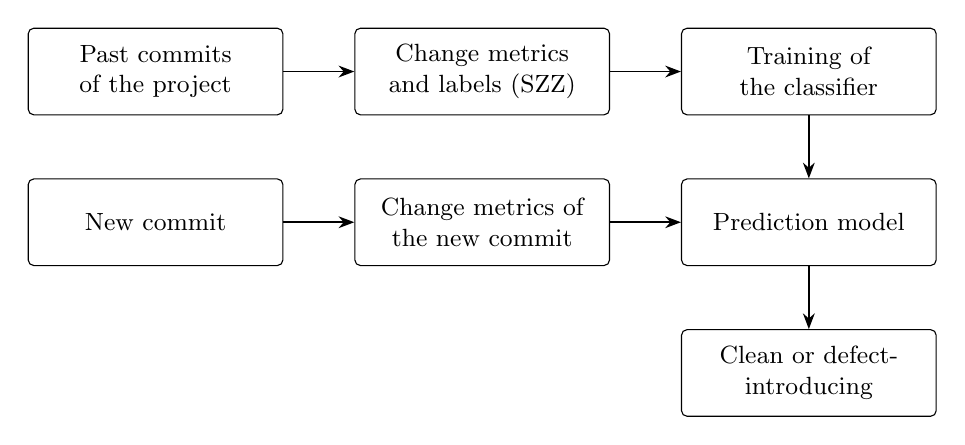
\begin{tikzpicture}[node distance=8mm and 9mm, font=\small,
  box/.style={draw, rounded corners=2pt, align=center, minimum height=11mm, text width=30mm},
  arr/.style={-{Stealth[length=2mm]}, semithick}]
\begin{scope}[every node/.append style={execute at begin node=\setstretch{1}}]
\node[box] (hist) {Past commits of the project};
\node[box, right=of hist] (feat) {Change metrics and labels (SZZ)};
\node[box, right=of feat] (train) {Training of the classifier};
\node[box, below=of train] (model) {Prediction model};
\node[box, left=of model] (newf) {Change metrics of the new commit};
\node[box, left=of newf] (new) {New commit};
\node[box, below=of model] (out) {Clean or defect-introducing};
\end{scope}
\draw[arr] (hist) -- (feat);
\draw[arr] (feat) -- (train);
\draw[arr] (train) -- (model);
\draw[arr] (new) -- (newf);
\draw[arr] (newf) -- (model);
\draw[arr] (model) -- (out);
\end{tikzpicture}
\caption{General workflow of just-in-time software defect prediction.}
\label{fig:workflow}
\end{figure}

Three characteristics of this task are important for the present work. First,
commits arrive one after another in time, so the data form a stream and the
model is always used on commits that are newer than the ones it was trained
on. Second, only a small fraction of the commits introduce defects. In the
dataset used in this work the fraction is 8.54\%, which means that the data
are highly imbalanced. Third, the label of a commit is not known when the
commit is made. It becomes known only later, when the defect is noticed and
fixed, and for a clean commit it is never confirmed at all.

\section{Labelling of Commits and the SZZ Algorithm}

To train a JIT-SDP model, every past commit needs a label that says whether
it introduced a defect. Software repositories do not store this information.
What can be found in a repository and its issue tracker is the set of commits
that \emph{fixed} defects, because developers normally mention the bug report
in the commit message. The commits that \emph{introduced} the defects have to
be inferred from these bug-fixing commits.

The standard method for this inference is the SZZ algorithm, proposed by
\'{S}liwerski, Zimmermann and Zeller~\cite{sliwerski2005szz}. The algorithm
takes a bug-fixing commit and looks at the lines that were deleted or modified
by it. For each of these lines it uses the annotation facility of the version
control system (\texttt{git blame}) to find the earlier commit in which the
line was last changed. These earlier commits are labelled as
defect-introducing. All commits that are never reached in this way are treated
as clean.

Figure~\ref{fig:szzexample} illustrates the procedure with a small example.
Commit $c_2$ adds a faulty line. The fault is corrected later in the
bug-fixing commit $c_5$. When SZZ traces the corrected line back, it reaches
$c_2$, which is the right answer. However, the developer of $c_5$ has also
edited another line that had nothing to do with the bug, for example to
improve the formatting. This line was last changed in $c_3$, so SZZ labels
$c_3$ as defect-introducing as well, although it is clean.

\begin{figure}[htbp]
\centering
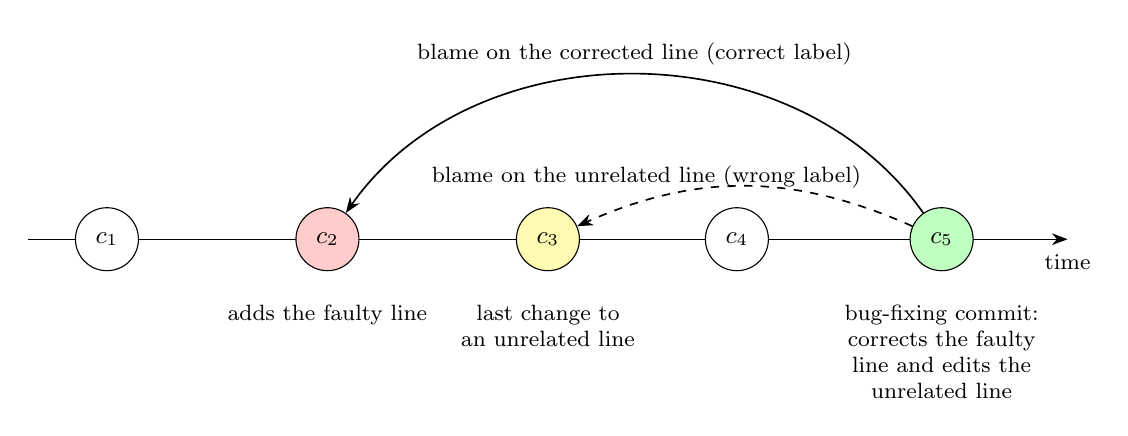
\begin{tikzpicture}[font=\small,
  c/.style={circle, draw, minimum size=8mm, inner sep=0pt},
  note/.style={align=center, font=\footnotesize, text width=27mm}]
\draw[-{Stealth[length=2mm]}] (0,0) -- (13.2,0) node[below=2pt, font=\footnotesize] {time};
\node[c, fill=white] (c1) at (1.0,0) {$c_1$};
\node[c, fill=red!20] (c2) at (3.8,0) {$c_2$};
\node[c, fill=yellow!30] (c3) at (6.6,0) {$c_3$};
\node[c, fill=white] (c4) at (9.0,0) {$c_4$};
\node[c, fill=green!25] (c5) at (11.6,0) {$c_5$};
\begin{scope}[every node/.append style={execute at begin node=\setstretch{1}}]
\node[note, below=3mm of c2] {adds the faulty line};
\node[note, below=3mm of c3] {last change to an unrelated line};
\node[note, below=3mm of c5] {bug-fixing commit: corrects the faulty line and edits the unrelated line};
\end{scope}
\draw[-{Stealth[length=2mm]}, semithick] (c5) to[bend right=55]
   node[above, font=\footnotesize] {blame on the corrected line (correct label)} (c2);
\draw[-{Stealth[length=2mm]}, semithick, dashed] (c5) to[bend right=24]
   node[above=1pt, font=\footnotesize, pos=0.8] {blame on the unrelated line (wrong label)} (c3);
\end{tikzpicture}
\caption{Example of how SZZ identifies defect-introducing commits and how a
change that is unrelated to the fix leads to a wrong label.}
\label{fig:szzexample}
\end{figure}

A bug-fixing commit that contains such unrelated modifications is called a
\emph{tangled} commit. Tangled commits are common. Herbold et
al.~\cite{herbold2022tangling} manually examined a large number of bug-fixing
commits and found that only 17\% to 32\% of the changed lines in them actually
contribute to the bug fix. The remaining lines are changes to tests,
documentation, formatting, refactoring and other modifications. Several
improved versions of SZZ have been proposed to remove such lines before the
blame step, and they are reviewed in Chapter~\ref{ch:lit}. It is important to
note that all of them still \emph{estimate} the label. None of the labels used
in JIT-SDP studies is directly observed.

\section{Motivation}

The motivation for this work comes from four issues in the way JIT-SDP models
are currently built and evaluated.

\paragraph{Noise in the SZZ labels.} Since the labels are produced by a
heuristic, some clean commits are labelled as defect-introducing (false
positives) and some defect-introducing commits are labelled as clean (false
negatives). A model trained on such labels learns partly from wrong examples.
Earlier studies have evaluated the accuracy of SZZ on small manually checked
samples~\cite{dacosta2017maszz,rosa2021oracle}, but the amount and the
type of noise over the complete history of a project, which is what a JIT-SDP
model is trained on, has received less attention.

\paragraph{Evaluation against the same noisy labels.} In nearly all JIT-SDP
studies the test set is labelled by the same SZZ implementation as the
training set. A model is therefore rewarded when it predicts what SZZ would
say, including the cases where SZZ is wrong. The reported performance then
measures how well the model reproduces the labelling heuristic, which is not
the same as how well it finds real defects. The difference between the two can
only be measured if labels from an independent source are available for
testing.

\paragraph{Evaluation that ignores time.} Many studies evaluate their models
with random $k$-fold cross-validation. On commit data this means that the
model may be trained on commits that were made after the commits on which it
is tested. Such a setting cannot occur in practice, and it has been shown for
defect prediction in general that it gives optimistic
results~\cite{falessi2020order,tan2015online}.

\paragraph{Delay in the arrival of labels.} Even when the commits are split
by time, it is normally assumed that the label of every training commit is
known at training time. In reality a defect-introducing commit is recognised
only when its defect is fixed, which may happen months or years later. Cabral
et al.~\cite{cabral2019orb} called this delay \emph{verification latency}.
During the delay the commit is treated as clean, so a model that is updated
continuously receives a wrong label first and the correct label later. The
delay can be long. Cabral and Minku~\cite{cabral2023reliable} report that the
time needed to discover a defect ranges from one day to more than eleven
years.

These four issues are related. The first one is about the quality of the
training data, and the other three are about the realism of the evaluation.
A study that wants to know how much the label noise matters in practice has to
control all of them at the same time.

\section{Problem Statement}

JIT-SDP models are trained and evaluated on labels generated by the SZZ
algorithm, and the evaluation is often carried out without respecting the
order of commits and the delay with which labels become available. As a
result, it is not known how much the errors made by SZZ reduce the ability of
a model to identify real defect-introducing commits when the model is used in
a realistic setting, and it is not possible to say how much of the performance
reported in the literature is due to the model and how much is due to the way
it was evaluated.

The problem addressed in this thesis is therefore to quantify the label noise
introduced by SZZ and its variants, to measure the effect of this noise on
JIT-SDP models under an evaluation that respects time order and verification
latency, and, in the later part of the thesis, to understand how the noise
affects an online learner and how its effect can be reduced.

The thesis work is divided into four stages. This report presents the work of
the first stage. It consists of the literature survey, the
identification of the research gaps, the formulation of the objectives and
research questions, the selection and description of the dataset, and the
design of the methodology. The work planned for the remaining stages is
described in Chapter~\ref{ch:conclusion}.

% ============================================================================
\chapter{Literature Review}\label{ch:lit}
% ============================================================================

This chapter reviews the literature related to the present work. It starts
with defect prediction in general and JIT-SDP in particular, then discusses
the SZZ algorithm and its variants, the studies on label noise, the evaluation
of prediction models, online learning for imbalanced data streams and learning
with noisy labels. A summary of the most closely related studies is given at
the end of the chapter.

\section{Software Defect Prediction}

Software defect prediction has been studied for more than three decades. The
usual approach is to describe each software module by a set of metrics, such
as size, complexity, coupling or the history of past changes, and to train a
classifier that separates defective modules from clean ones. Hall et
al.~\cite{hall2012slr} carried out a systematic review of 208 fault prediction
studies and observed that models based on simple techniques such as Na\"ive
Bayes and logistic regression often perform as well as more complex ones, and
that the quality of the data and of the experimental procedure has a large
influence on the reported results. Rathore and Kumar~\cite{rathore2019study}
reviewed the field with respect to three aspects: the software metrics used,
the prediction techniques and the data quality issues. Among the data quality
issues they discuss class imbalance and noise in the data, both of which are
central to the present work.

Most of this research predicts defects for files, classes or modules of a
given release. The limitations of this granularity, mentioned in
Chapter~\ref{ch:intro}, led to the prediction of defects at the level of
individual changes.

\section{Just-in-Time Software Defect Prediction}

\subsection{Change-level prediction and change metrics}

Mockus and Weiss~\cite{mockus2000risk} were among the first to predict the
risk of a software change. They used properties of the change, such as its
size, the number of files and subsystems it touches, the experience of the
developer and the type of the change, to predict the probability that a change
to a large telecommunication system would cause a failure. Kim et
al.~\cite{kim2008classifying} introduced \emph{change classification}, in
which a classifier is trained to decide whether a change is buggy or clean.
They used features extracted from the change log, the source code and the
change metadata, and obtained on average 78\% accuracy and 60\% recall for
buggy changes on twelve open-source projects.

Kamei et al.~\cite{kamei2013jit} carried out a large empirical study on six
open-source and five commercial projects and introduced the term
``just-in-time'' for this kind of quality assurance. They proposed fourteen
change metrics that are grouped into five dimensions: diffusion, size,
purpose, history and experience. Their logistic regression model predicted
defect-inducing changes with an average accuracy of 68\% and a recall of 64\%.
These fourteen metrics have become the standard feature set for JIT-SDP and
are also used in the present work. They are described in detail in
Section~\ref{sec:features}. A recent survey by Zhao et
al.~\cite{zhao2023survey} covers 67 JIT-SDP studies and shows that the
majority of them follow the formulation of Kamei et al.\ with respect to both
the features and the way the labels are obtained.

McIntosh and Kamei~\cite{mcintosh2018moving} studied how JIT-SDP models
behave over time on the Qt and OpenStack projects. They found that the
properties of defect-inducing changes are not stable. The importance of the
different metrics changes as a project evolves, and a model loses a
considerable part of its predictive power when it is used long after it was
trained. This result shows that time has to be taken into account both in
training and in evaluating such models.

\subsection{Learning techniques}

A wide range of learning techniques has been applied to JIT-SDP. Besides
logistic regression, random forests and other ensemble methods are frequently
used. More recently, deep learning models have been proposed that learn
features directly from the content of a change. DeepJIT~\cite{hoang2019deepjit}
applies convolutional networks to the commit message and to the changed code.
CC2Vec~\cite{hoang2020cc2vec} learns a vector representation of a code change
with a hierarchical attention network and combines it with DeepJIT.

Later studies have questioned whether this additional complexity is
necessary. Zeng et al.~\cite{zeng2021lapredict} replicated DeepJIT and CC2Vec
on a larger dataset of more than 310,000 changes. They reported that the deep
models did not consistently perform better than traditional approaches, and
that a logistic regression model using only the number of added lines, which
they called LApredict, outperformed both of them in most cases while being
many times faster. Pornprasit and
Tantithamthavorn~\cite{pornprasit2021jitline} proposed JITLine, which uses a
random forest together with oversampling of the minority class, and showed
that it is more accurate and much faster than the deep models. Yang et
al.~\cite{yang2016effort} had earlier shown for effort-aware prediction that
simple unsupervised models built from a single change metric can be better
than supervised models.

These studies are relevant here for two reasons. First, they show that the
ranking of models in JIT-SDP depends strongly on how the evaluation is done.
Second, they provide two well-known models of very different complexity,
LApredict and JITLine, which will be used in the present work to examine whether
the effect of label noise depends on the capacity of the model.

\section{Identification of Defect-Introducing Changes}

\subsection{The SZZ algorithm}

The SZZ algorithm~\cite{sliwerski2005szz} consists of two phases. In the
first phase, bug-fixing commits are identified by linking the commits of the
version control system to the reports in the bug tracking system, mainly by
searching the commit messages for bug identifiers. In the second phase, for
every bug-fixing commit the lines that were deleted or modified are
determined, and the annotate (blame) command is used to find the most recent
earlier commits that changed these lines. Commits that were made after the bug
was reported are excluded, since they cannot have caused the bug. The
remaining commits are considered to be bug-introducing.

The algorithm depends on two assumptions. The first is that the lines changed
by the fix are the lines that contained the defect. The second is that the
commit that last changed such a line is the commit that made it defective.
Both assumptions can fail. The first one fails for tangled commits, where
some of the changed lines are not related to the fix. The second one fails
when a line was last touched by a cosmetic change, such as a renaming or
re-indentation, so that the blame points to this change instead of the
original faulty one. In addition, a defect that is fixed only by adding new
lines leaves no deleted or modified line to trace, and a defect caused by a
change in the environment or in the requirements has no introducing commit in
the repository at all~\cite{rodriguez2020bugs}.

\subsection{Variants of SZZ}

Several variants have been proposed to reduce the number of wrong labels
produced by the original algorithm, which is usually called B-SZZ (basic
SZZ). Table~\ref{tab:variants} lists the variants that are studied in this
work.

\begin{table}[htbp]
\centering\small
\caption{SZZ variants considered in this work.}
\label{tab:variants}
\begin{tabularx}{\linewidth}{@{}l>{\raggedright\arraybackslash}X@{}}
\toprule
Variant & Main idea \\
\midrule
B-SZZ~\cite{sliwerski2005szz} & Original algorithm. Every line deleted or
modified by the bug-fixing commit is traced back with blame. \\
AG-SZZ~\cite{kim2006agszz} & Uses an annotation graph to follow lines across
revisions and ignores blank lines, comments and formatting changes. \\
MA-SZZ~\cite{dacosta2017maszz} & Builds on AG-SZZ and additionally ignores
meta-changes, i.e.\ branch changes, merge changes and property changes, which
do not modify the source code. \\
R-SZZ~\cite{davies2014rlszz} & Builds on MA-SZZ and keeps, for each bug-fixing
commit, only the most recent of the candidate commits. \\
L-SZZ~\cite{davies2014rlszz} & Builds on MA-SZZ and keeps only the candidate
commit that changed the largest number of lines. \\
RA-SZZ~\cite{neto2018raszz} & Builds on MA-SZZ and ignores lines that were
changed by refactoring operations, which are detected with a refactoring
detection tool. It is available for Java only. \\
\bottomrule
\end{tabularx}
\end{table}

Kim et al.~\cite{kim2006agszz} observed that many lines changed in a
bug-fixing commit are comments, blank lines or formatting changes and proposed
to ignore them. They also replaced the simple annotate command by an
annotation graph, which follows a line more reliably when code is moved. Da
Costa et al.~\cite{dacosta2017maszz} noticed that some commits flagged by SZZ
are only changes to the repository structure, such as merges, and excluded
these meta-changes. R-SZZ and L-SZZ go one step further and select a single
commit from the candidates returned for a bug-fixing
commit~\cite{davies2014rlszz}. They assume that a bug has one introducing
commit and choose either the latest or the largest candidate. Neto et
al.~\cite{neto2018raszz} showed that refactoring operations are a frequent
cause of wrong labels and proposed RA-SZZ, which removes refactored lines
from the analysis.

All these variants try to reduce false positives by removing lines or
candidate commits. An obvious consequence, which will be examined in this
thesis, is that some correct candidates may be removed as well.

\subsection{Empirical evaluations of SZZ}

The accuracy of SZZ is difficult to evaluate, because the true
defect-introducing commits are not known. Da Costa et
al.~\cite{dacosta2017maszz} proposed a framework that evaluates SZZ
implementations indirectly through three criteria: the earliest appearance of
the bug, the future impact of the flagged changes and the realism of the bug
introduction. They applied it to five implementations on ten open-source
projects and found that the existing implementations still have considerable
room for improvement.

Rodr\'{\i}guez-P\'{e}rez et al.~\cite{rodriguez2018szz} reviewed 187 papers
that use SZZ and found that most of them neither discuss the limitations of
the algorithm nor provide enough detail to reproduce the labelling. In a later
study~\cite{rodriguez2020bugs} they manually analysed how 116 bugs were
introduced in two open-source projects. They found that a part of the bugs
are \emph{extrinsic}, i.e.\ caused by changes outside the project code, and
that the SZZ-based algorithms reached F-scores of only 0.44 to 0.77 on the
remaining ones.

Rosa et al.~\cite{rosa2021oracle,rosa2023szzvariants} built a
\emph{developer-informed oracle} from commit messages in which the developer
explicitly names the commit that introduced the bug being fixed. The oracle
contains 1,930 such cases, extended to 2,304 in the journal version, and was
used to compare several SZZ variants. R-SZZ obtained the best results, with a
precision of about 66\% and an F-measure of about 61\%, while B-SZZ had a
higher recall but a precision of only about 39\%. The authors also released
PySZZ, an open-source implementation of the variants, which will be used in
the present work.

Two properties of this oracle are important for the present study. It
contains only bug-fixing commits together with their introducing commits and
no clean commits, so it cannot be used to train or test a JIT-SDP model. It
also evaluates SZZ only on fixes for which an introducing commit is known to
exist. This is a different question from the one that matters for JIT-SDP,
where every commit in the history of the project receives a label.

\subsection{Tangled changes}

Herzig and Zeller~\cite{herzig2013tangled} studied tangled changes in five
open-source Java projects and found that up to 15\% of the bug fixes consist
of several unrelated changes. As a result, at least 16.6\% of the source files
were incorrectly associated with bug reports. Herbold et
al.~\cite{herbold2022tangling} conducted a large crowd-sourced study in which
every changed line of the bug-fixing commits of several Apache projects was
labelled by four participants. They found that only 17\% to 32\% of all
changed lines contribute to the bug fix. When only changes to production code
files are considered, the share is 66\% to 87\%. For about 11\% of the lines
the participants could not agree on a label. The dataset produced by this
study, called LLTC4J, is the basis of the reference labels used in the present
work (Section~\ref{sec:reference}).

\section{Label Noise in Defect Prediction}

The effect of wrong labels on defect prediction models has been studied
mainly for file-level prediction. Kim et al.~\cite{kim2011noise} added
artificial false positive and false negative noise to defect datasets and
found that the prediction performance decreases significantly once the
datasets contain about 20\% to 35\% of both types of noise. They also proposed
a method to detect and remove noisy instances. Tantithamthavorn et
al.~\cite{tantithamthavorn2015mislabelling} examined mislabelling that arises
from wrongly classified issue reports. They showed that such mislabelling is
not random, and that models trained on the noisy data keep their precision
but reach only 56\% to 68\% of the recall of models trained on clean data.

For JIT-SDP, the most closely related study is that of Fan et
al.~\cite{fan2021mislabeled}. They labelled 126,526 changes from ten Apache
projects with four SZZ variants (B-SZZ, AG-SZZ, MA-SZZ and RA-SZZ) and
examined how the differences between the variants affect JIT-SDP models. They
reported that the changes mislabelled by B-SZZ and MA-SZZ do not reduce the
prediction performance considerably, whereas those mislabelled by AG-SZZ lead
to a statistically significant reduction. Since no ground truth was available,
they treated the labels of RA-SZZ as correct and measured the mislabelling of
the other variants relative to it. This has two consequences. The noise of
RA-SZZ itself could not be measured, and errors that are common to all
variants, for example those caused by tangled changes, remained invisible. The
study also did not consider the delayed arrival of labels.

\section{Evaluation of Defect Prediction Models}

\subsection{Validation schemes and time order}

Cross-validation with random folds is the most common validation scheme in
defect prediction. For data that are ordered in time it has a known weakness,
because a model can be trained on data that are newer than the test data. Tan
et al.~\cite{tan2015online} pointed out for change classification that
cross-validation uses information from the future and can therefore report a
precision that is too high. They proposed a time-sensitive evaluation in
which the model is trained only on changes that precede the test changes.
Falessi et al.~\cite{falessi2020order} analysed this issue systematically for
within-project defect classifiers. They showed that validation techniques
which do not preserve the order of the data produce results that differ from
those of order-preserving techniques, and recommended the latter. In spite of
these findings, random cross-validation is still widely used in JIT-SDP
studies~\cite{zhao2023survey}.

\subsection{Prequential evaluation}

When data arrive as a stream, the standard evaluation procedure is
\emph{prequential} (predictive sequential) evaluation, also known as
test-then-train. Each example is first used to test the model and afterwards
to update it. The performance is accumulated over the stream. Since the
performance at the beginning of the stream is often poor and less relevant, a
forgetting mechanism such as a sliding window or a fading factor is applied.
Gama et al.~\cite{gama2013prequential} showed that the prequential error
computed with a fading factor converges to the same value as the error on an
independent holdout set. This result holds for the error rate. For measures
that are computed from the complete confusion matrix, such as MCC, no
corresponding result is available, which has to be kept in mind when
prequential values of such measures are summarised.

\subsection{Verification latency}

Cabral et al.~\cite{cabral2019orb} were the first to investigate JIT-SDP as an
online learning problem with verification latency. In their setting a commit
is used as a clean training example when a waiting period has passed without
a defect being linked to it, and as a defect-inducing example as soon as a
defect is linked to it. They used a waiting period of 90 days. They showed
that, because of this mechanism, the proportion of the two classes seen by
the learner changes over time, which they called class imbalance evolution,
and that this hinders the existing approaches. To deal with it they proposed
the ORB method, which is described in Section~\ref{sec:lit-online}. In a later
study, Cabral and Minku~\cite{cabral2023reliable} examined concept drift in
JIT-SDP in more detail. They reported that the time needed to discover a
defect ranges from one day to more than eleven years, and proposed a method
that also uses the predictions on unlabelled commits to detect when the model
has become unreliable. Tabassum et al.~\cite{tabassum2020cross} studied the
use of data from other projects in the same online setting.

In these studies the wrong labels that the learner receives are caused by
time: a defect-introducing commit is treated as clean until its defect is
found. The labels that finally arrive are assumed to be correct. The noise
that comes from the SZZ algorithm itself, where the final label is wrong and
is never corrected, is not addressed.

\subsection{Performance measures}

Because the classes are imbalanced, accuracy is not a suitable measure for
defect prediction. Precision, recall and the F-measure are widely used, but
the F-measure ignores the true negatives and depends on the proportion of the
positive class. Yao and Shepperd~\cite{yao2020mcc} showed that the use of the
F-measure can lead to different conclusions than the Matthews correlation
coefficient (MCC)~\cite{matthews1975mcc} in a considerable number of defect
prediction comparisons and recommended MCC. Chicco and
Jurman~\cite{chicco2020mcc} reached the same recommendation for binary
classification in general. MCC uses all four cells of the confusion matrix
and takes the value zero for a classifier that predicts at random or always
predicts the same class. For measuring the agreement between two sets of
labels, Cohen's $\kappa$~\cite{cohen1960kappa} is commonly used, which
corrects the observed agreement for the agreement expected by chance. Landis
and Koch~\cite{landis1977kappa} proposed the widely used verbal
interpretation of $\kappa$ values, according to which values up to 0.20
indicate slight agreement and values above 0.80 almost perfect agreement.

\section{Online Learning for Imbalanced Data Streams}\label{sec:lit-online}

Online Bagging~\cite{oza2001onlinebagging} is the online version of the
bagging ensemble. In ordinary bagging each base learner is trained on a
bootstrap sample of the data. In the online version, each arriving example is
presented to each base learner $k$ times, where $k$ is drawn from a Poisson
distribution with parameter $\lambda = 1$. Wang et al.~\cite{wang2015oob}
adapted this method to imbalanced streams. In their Oversampling Online
Bagging (OOB), the parameter $\lambda$ for an example of the minority class
is increased according to the current ratio of the class sizes, so that
minority examples are presented more often. The class sizes are tracked with
a time-decayed average, which allows the method to follow changes in the
imbalance.

ORB (Oversampling Rate Boosting)~\cite{cabral2019orb} extends OOB for
JIT-SDP. It monitors the predictions that the model has made recently. If the
model predicts one class much more often than expected, the resampling rate
of the other class is increased further by a boosting factor. In this way the
model is pushed back when it becomes biased towards one class, which happens
frequently under verification latency.

It should be noted that in all these methods the resampling rate depends only
on how many examples of each class have been observed. Whether the labels of
these examples are correct plays no role. A commit that is wrongly labelled
as defect-introducing is oversampled in the same way as a correctly labelled
one. This property is one of the reasons why the effect of label noise on
such learners deserves to be studied.

\section{Learning with Noisy Labels}

In the machine learning literature, several methods have been proposed for
training classifiers on data with wrong labels. Natarajan et
al.~\cite{natarajan2013noisy} considered the case where the probability that
a label is flipped depends on the class, which is called class-conditional
noise. They showed that, if the two flip rates are known, the loss function
can be modified such that minimising it on the noisy data is equivalent in
expectation to minimising the original loss on clean data. The correction
contains the factor $1/(1-\rhoz-\rhoo)$, where $\rhoz$ and $\rhoo$ are the
two flip rates, and becomes unstable when the sum of the rates approaches
one. Co-teaching~\cite{han2018coteaching} trains two neural networks at the
same time. Each network selects the examples with small loss in a mini-batch,
which are likely to be correctly labelled, and passes them to the other
network for training. Confident learning~\cite{northcutt2021confident}
estimates the joint distribution of the given and the true labels from the
predicted probabilities of a classifier and uses it to identify and remove
the examples that are probably mislabelled.

These methods were developed for the batch setting, in which the complete
dataset is available and can be processed several times. They also assume
that a wrong label stays wrong. In online JIT-SDP each example is seen once,
its label arrives late, and a label may be changed later from clean to
defect-introducing. The methods can therefore not be applied directly, but
the class-conditional noise model on which they are based is the one that
will be measured in the present work.

\section{Summary}

Table~\ref{tab:litsummary} summarises the studies that are most closely
related to the present work and indicates in which respect each of them
differs from it. The review shows that the accuracy of SZZ, the effect of
label noise, time-aware evaluation and verification latency have each been
studied, but mostly in isolation. The gaps that follow from this are stated
in the next chapter.

\begin{table}[htbp]
\centering\footnotesize
\setlength{\tabcolsep}{4pt}
\caption{Summary of the most closely related studies.}
\label{tab:litsummary}
\begin{tabularx}{\linewidth}{@{}>{\raggedright\arraybackslash}p{27mm}>{\raggedright\arraybackslash}p{40mm}>{\raggedright\arraybackslash}X@{}}
\toprule
Study & Focus & Difference from the present work \\
\midrule
Kamei et al.~\cite{kamei2013jit} & Change metrics and models for JIT-SDP &
Labels from SZZ are taken as correct; no time-aware evaluation \\
Da Costa et al.~\cite{dacosta2017maszz} & Framework for evaluating SZZ
implementations & Indirect criteria; effect on prediction models not studied \\
Rosa et al.~\cite{rosa2021oracle,rosa2023szzvariants} & Accuracy of SZZ
variants against a developer-informed oracle & Oracle has no clean commits;
effect on prediction models not studied \\
Herbold et al.~\cite{herbold2022tangling} & Amount of tangling in bug-fixing
commits & Line-level analysis; labels of commits and models not studied \\
Kim et al.~\cite{kim2011noise} & Artificial label noise in file-level defect
data & Noise is injected artificially; file-level prediction with batch evaluation \\
Fan et al.~\cite{fan2021mislabeled} & Effect of labels of four SZZ variants on
JIT-SDP & RA-SZZ used as reference; no independent labels; no latency \\
Falessi et al.~\cite{falessi2020order} & Order-preserving validation of defect
classifiers & Label noise not considered \\
Cabral et al.~\cite{cabral2019orb} & Online JIT-SDP with verification latency
and class imbalance evolution & SZZ labels taken as correct once they arrive \\
Zeng et al.~\cite{zeng2021lapredict} & Comparison of deep and simple JIT-SDP
models & Label noise and latency not considered \\
Natarajan et al.~\cite{natarajan2013noisy} & Learning under class-conditional
label noise & Batch setting; noise rates assumed to be known \\
\bottomrule
\end{tabularx}
\end{table}

% ============================================================================
\chapter{Research Gaps, Objectives and Research Questions}\label{ch:gaps}
% ============================================================================

This chapter states the research gaps that were identified from the
literature reviewed in Chapter~\ref{ch:lit}. Based on these gaps, the
objectives of the thesis are formulated, and the research questions that
follow from them are stated. The stage of the thesis in which each of them
will be addressed is indicated.

\section{Research Gaps}

The following gaps were identified.

\paragraph{Gap 1: The noise of SZZ labels has not been measured over complete
project histories.} The existing evaluations of SZZ either use indirect
criteria~\cite{dacosta2017maszz} or check the algorithm on a sample of
bug-fixing commits for which the introducing commit is
known~\cite{rosa2021oracle,rodriguez2020bugs}. These evaluations tell how
often SZZ finds the right commit for a given fix. They do not tell how many
of the commits in the history of a project receive a wrong label, which is
the quantity that matters for a JIT-SDP model, because the model is trained on
all commits. In particular, the rate of false positives among the clean
commits and the rate of false negatives among the defect-introducing commits
have not been reported separately for the different variants.

\paragraph{Gap 2: Models are tested against the same labels on which they are
trained.} In the JIT-SDP literature the test labels come from the same SZZ
implementation as the training labels. The study that is closest to the
present work~\cite{fan2021mislabeled} used one SZZ variant as the reference
for the others. Hence it is not known how well a model that was trained on
SZZ labels predicts labels that were obtained independently of the SZZ
variant used for training.

\paragraph{Gap 3: The effect of label noise has not been separated from the effect
of the evaluation procedure.} It is known that random cross-validation gives
optimistic results for time-ordered
data~\cite{falessi2020order,tan2015online}, and it is known that SZZ labels
contain errors. These two factors are present together in most published
results, and their individual contributions have not been measured in a
common experimental design.

\paragraph{Gap 4: Label noise has not been studied under verification latency.}
The studies on online JIT-SDP~\cite{cabral2019orb,cabral2023reliable} model
the delay of the labels but assume that the labels which finally arrive are
correct. The studies on label noise use batch
evaluation~\cite{kim2011noise,fan2021mislabeled}. The loss caused by SZZ
noise for an online learner that receives delayed labels is therefore not
known.

\paragraph{Gap 5: The way in which SZZ noise affects an online learner is not
understood, and no remedy designed for this setting exists.} Online learners
for imbalanced streams oversample the minority class according to the number
of positive labels they observe (Section~\ref{sec:lit-online}), without
regard to their correctness. Whether false positives or false negatives are
more harmful for such learners is not known. The existing methods for
learning with noisy labels assume a batch setting and stable
labels~\cite{natarajan2013noisy,northcutt2021confident} and cannot be applied
directly to a stream with delayed labels.

\section{Objectives}

Based on these gaps, the main objectives of the thesis are as follows.

\begin{enumerate}[leftmargin=*]
\item To quantify the label noise introduced by SZZ and its variants, by
comparing their labels with independently obtained reference labels over
complete project histories.
\item To measure the effect of this noise on JIT-SDP models under a realistic
evaluation, in which the order of the commits and the delay of the labels are
respected, and to separate it from the effect of the evaluation procedure.
\item To identify how the noise affects an online learner, and to develop a
noise-aware online learning approach that reduces its effect.
\end{enumerate}

Objectives 1 and 2 will be addressed in the second stage of the thesis.
Objective 3 will be addressed in the third and fourth stages. The plan of
work is given in Section~\ref{sec:plan}.

\section{Research Questions}

To meet these objectives, the following research questions will be answered.

\paragraph{RQ1: How much do the labels of different SZZ variants disagree with one
another and with independently obtained reference labels, and what type of
error does each variant make?}
This question belongs to Objective~1 and corresponds to Gap~1. To answer it,
the labels of six SZZ variants will be compared with reference labels on the
same set of commits, and the false positive and false negative rates of each
variant will be estimated.

\paragraph{RQ2: How does the choice of the label source affect the measured
performance of JIT-SDP models under different evaluation settings?}
This question belongs to Objective~2 and corresponds to Gaps~2, 3 and~4. To
answer it, models will be trained on the reference labels and on the labels
of each SZZ variant, and will be evaluated with random cross-validation, with
a chronological split and with prequential evaluation under verification
latency. The predictions will be scored against the reference labels and,
for comparison, against the training labels.

\paragraph{RQ3: Through which mechanism does label noise reduce the performance of
an online learner, and which of the two types of error is responsible?}
This question belongs to Objective~3 and corresponds to the first part of
Gap~5. It will be addressed in the third stage.

\paragraph{RQ4: Can an online learner be modified so that it loses less
performance when it is trained on SZZ labels, without access to clean labels
and without losing performance when the labels are clean?}
This question also belongs to Objective~3 and corresponds to the second part
of Gap~5. It will be addressed in the fourth stage.

% ============================================================================
\chapter{Dataset}\label{ch:data}
% ============================================================================

This chapter describes the dataset used in the study. It first states the
requirements that the dataset has to satisfy and then describes the
JIT-Defects4J dataset, the projects it contains, the reference labels, the
change metrics and the preparation of the data.

\section{Requirements}

The research questions place several requirements on the dataset.

\begin{itemize}[leftmargin=*]
\item A label must be available for every commit of a project, including the
clean commits, because JIT-SDP models are trained and tested on the complete
commit history.
\item The labels must not have been produced by the SZZ variant that is being
evaluated. Otherwise the errors of that variant cannot be observed.
\item The change metrics of the commits must be available, so that prediction
models can be trained.
\item The repositories of the projects must be accessible, because the SZZ
variants have to be executed on them and the dates of the bug-fixing commits
are needed for simulating verification latency.
\item The dataset should contain several projects, so that the comparisons
can be tested statistically across projects.
\end{itemize}

Most JIT-SDP datasets do not satisfy the second requirement.
ApacheJIT~\cite{keshavarz2022apachejit}, which contains 106,674 commits, and
Defectors~\cite{mahbub2023defectors} are much larger than the dataset used
here, but their labels were generated with SZZ. The developer-informed oracle
of Rosa et al.~\cite{rosa2021oracle} does not satisfy the first requirement,
since it contains no clean commits. The JIT-Defects4J dataset satisfies all
five requirements and was therefore selected.

\section{The JIT-Defects4J Dataset}

JIT-Defects4J was published by Ni et al.~\cite{ni2022jitdefects4j} together
with their JIT-Fine approach. It was built from LLTC4J, the dataset of Herbold
et al.~\cite{herbold2022tangling}, in which the changed lines of bug-fixing
commits were labelled manually. JIT-Defects4J contains 27,319 commits from 21
open-source Java projects of the Apache Software Foundation. For every commit
it provides the fourteen change metrics of Kamei et al.\ and a label that
indicates whether the commit introduced a defect. The dataset was used as it
was published. No project was added or removed, so the selection of projects
could not be influenced by the results of this study.

\section{Subject Projects}

Table~\ref{tab:projects} lists the 21 projects. Sixteen of them are libraries
of the Apache Commons family. The other five are a dependency manager
(ant-ivy), a graph processing system (giraph), a data persistence framework
(gora), a natural language processing toolkit (opennlp) and a columnar storage
format (parquet-mr). The commits were made between 2001 and 2019. The length
of the covered history of a project varies from about 6 years (parquet-mr) to
about 18 years (commons-dbcp).

\begin{table}[htbp]
\centering\small
\caption{Projects of the JIT-Defects4J dataset. The last two columns give the
number and the percentage of defect-introducing commits according to the
reference labels.}
\label{tab:projects}
\begin{tabular}{@{}lcrrrr@{}}
\toprule
Project & Period & Commits & Bug-fixing & \multicolumn{2}{c}{Defect-introducing} \\
\cmidrule(l){5-6}
 & & & commits & Number & \% \\
\midrule
ant-ivy & 2005--2018 & 1,771 & 761 & 332 & 18.7 \\
commons-bcel & 2001--2019 & 825 & 134 & 60 & 7.3 \\
commons-beanutils & 2001--2018 & 611 & 197 & 37 & 6.1 \\
commons-codec & 2003--2018 & 761 & 122 & 36 & 4.7 \\
commons-collections & 2001--2018 & 1,823 & 360 & 50 & 2.7 \\
commons-compress & 2003--2018 & 1,630 & 175 & 178 & 10.9 \\
commons-configuration & 2003--2018 & 1,838 & 358 & 155 & 8.4 \\
commons-dbcp & 2001--2019 & 1,037 & 348 & 58 & 5.6 \\
commons-digester & 2001--2017 & 1,079 & 221 & 19 & 1.8 \\
commons-io & 2002--2018 & 1,142 & 224 & 73 & 6.4 \\
commons-jcs & 2002--2018 & 831 & 237 & 88 & 10.6 \\
commons-lang & 2002--2018 & 2,969 & 491 & 146 & 4.9 \\
commons-math & 2003--2018 & 4,026 & 758 & 335 & 8.3 \\
commons-net & 2002--2018 & 1,121 & 197 & 117 & 10.4 \\
commons-scxml & 2005--2018 & 544 & 55 & 47 & 8.6 \\
commons-validator & 2002--2018 & 598 & 120 & 36 & 6.0 \\
commons-vfs & 2002--2018 & 1,110 & 201 & 114 & 10.3 \\
giraph & 2010--2018 & 844 & 118 & 163 & 19.3 \\
gora & 2010--2019 & 553 & 85 & 39 & 7.1 \\
opennlp & 2010--2018 & 1,086 & 83 & 91 & 8.4 \\
parquet-mr & 2012--2018 & 1,120 & 208 & 158 & 14.1 \\
\midrule
Total & & 27,319 & 5,453 & 2,332 & 8.54 \\
\bottomrule
\end{tabular}
\end{table}

In total, 5,453 commits (20.0\%) are marked as bug-fixing and 2,332 commits
(8.54\%) are defect-introducing according to the reference labels. The
projects differ considerably in size and in the proportion of
defect-introducing commits, as can be seen in Figure~\ref{fig:projects}. The
smallest project has 544 commits and the largest has 4,026. The number of
defect-introducing commits ranges from 19 in commons-digester to 335 in
commons-math, and the defect rate ranges from 1.8\% to 19.3\%. In every
project the defect-introducing commits are a clear minority. Because of these
differences, all comparisons in this work will be made project by project,
and the results will then be summarised over the projects.

\begin{figure}[htbp]
\centering
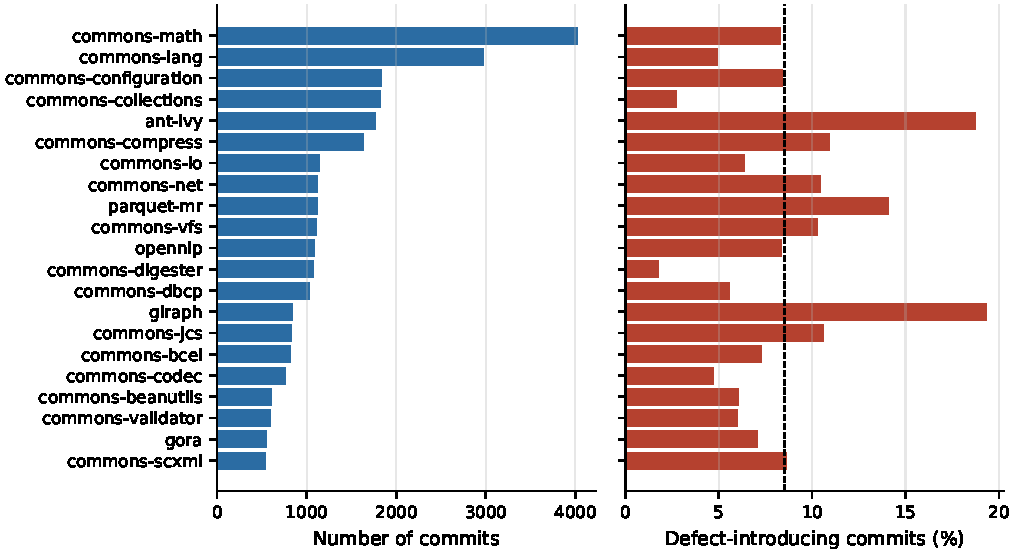
\includegraphics[width=0.95\linewidth]{fig_projects}
\caption{Number of commits and percentage of defect-introducing commits in
each project. The dashed line marks the percentage in the whole dataset
(8.54\%).}
\label{fig:projects}
\end{figure}

\section{Reference Labels}\label{sec:reference}

The label provided with JIT-Defects4J will be used in this work as the
reference against which the SZZ variants and the predictions of the models
are assessed. Since all later results will depend on this label, its
construction is described in detail.

According to the description given by the authors of the
dataset~\cite{ni2022jitdefects4j}, the labels were obtained in two steps. In
the first step, they took the bug-fixing commits of LLTC4J. In LLTC4J every
changed line of a bug-fixing commit was labelled by four participants, and a
line is regarded as contributing to the bug fix only if at least three of
them assigned this label. In the second step, \texttt{git blame} was applied
to each of these validated lines to find the commit that introduced it. The
commits found in this way are the defect-introducing commits. All other
commits are considered clean.

To make sure that the labels in the files obtained for this work are indeed
these labels, the number of commits and of defect-introducing commits of
every project was compared with the numbers reported in the paper. They agree
for all 21 projects.

The reference labels are thus the result of the blame operation applied to
manually validated bug-fixing lines. They are not a manual judgement about
each commit. This has the following consequences for the interpretation of
the results.

\begin{enumerate}[leftmargin=*]
\item The reference labels and the SZZ labels differ in the lines from which
the tracing starts. SZZ starts from all lines changed in a bug-fixing commit
(after the filtering applied by the particular variant), whereas the reference
starts only from the lines that were confirmed to be part of the fix. A
comparison between the two therefore shows the effect of tangled changes, and
of the filters that the variants use to deal with them.
\item Both use the blame operation to go from a line to a commit. Errors of
the blame operation itself, for example when a line was last touched by a
cosmetic change, are present in both and cannot be detected by comparing
them. The amount of noise that will be measured in this work should therefore
be regarded as a lower bound of the true amount.
\item Every commit that is defect-introducing according to the reference can
be reached by blame from some line of a bug-fixing commit. When an SZZ
variant misses such a commit, the reason cannot be that blame is unable to
reach it. The reason must lie in the lines selected or in the filtering of the
candidates.
\item The authors of the dataset excluded changes that do not add any line.
Defects that are introduced only by deleting code are therefore not
represented.
\end{enumerate}

In the rest of this report the term \emph{reference labels} is used for these
labels. The term ``ground truth'' is avoided, because the labels are more
reliable than SZZ labels with respect to tangling but are not free of error.

\section{Change Metrics}\label{sec:features}

Each commit is described by the fourteen change metrics proposed by Kamei et
al.~\cite{kamei2013jit}. They are listed in Table~\ref{tab:metrics}. The
metrics of the diffusion group measure how widely a change is spread over the
code base, since changes that touch many parts are more difficult to
understand. The size group measures how much code was changed. The purpose
group contains a single metric which indicates whether the change is a bug
fix, since bug fixes are known to introduce new defects more often than other
changes. The history group describes how the modified files were changed in
the past, and the experience group describes how familiar the developer is
with the project and with the modified subsystem.

\begin{table}[htbp]
\centering\small
\caption{The fourteen change metrics used as features~\cite{kamei2013jit}.}
\label{tab:metrics}
\begin{tabularx}{\linewidth}{@{}llX@{}}
\toprule
Group & Metric & Description \\
\midrule
Diffusion & NS & Number of modified subsystems \\
 & ND & Number of modified directories \\
 & NF & Number of modified files \\
 & Entropy & Distribution of the modified code across the files \\
\midrule
Size & LA & Lines of code added \\
 & LD & Lines of code deleted \\
 & LT & Lines of code in the files before the change \\
\midrule
Purpose & FIX & Whether the change is a defect fix \\
\midrule
History & NDEV & Number of developers that changed the modified files \\
 & AGE & Average time interval between the last and the current change \\
 & NUC & Number of unique changes to the modified files \\
\midrule
Experience & EXP & Number of changes made by the developer so far \\
 & REXP & Recent experience of the developer (changes weighted by their age) \\
 & SEXP & Experience of the developer on the modified subsystem \\
\bottomrule
\end{tabularx}
\end{table}

The values of the metrics were taken from the dataset as published and were
not recomputed. In this way the features are identical for all label sources,
and differences between the results obtained with different labels cannot be
caused by differences in feature extraction. Several of the metrics have
strongly skewed distributions. Suitable transformations will be applied to
them when the prediction models are trained.

\section{Data Preparation}

The dataset is distributed in three files that correspond to the training,
validation and test split used by its authors. These files were merged, since
the present work uses its own evaluation settings. Duplicate records were
removed on the combination of project and commit identifier. Within each
project the commits were sorted by their author timestamp. This order defines
the commit stream of the project and is used in all evaluation settings that
depend on time.

The repositories of the 21 projects were also cloned from GitHub. They will be
needed in the second stage to run the SZZ variants and to obtain the dates of the
bug-fixing commits.

\section{Information to be Added to the Dataset}\label{sec:additions}

The dataset provides one label for each commit, the reference label. For the
purpose of this thesis two kinds of information have to be added to it. Both
will be produced in the second stage of the thesis.

The first is the set of SZZ labels. To study the noise of SZZ, six further
labels will be attached to every commit, one for each SZZ variant of
Table~\ref{tab:variants}. They will be generated by running the variants on
the repositories of the 21 projects, with the bug-fixing commits of the
dataset as input (Section~\ref{sec:szz-generation}). Each commit will then
have seven binary labels.

The second is the time at which the label of each commit becomes available.
To evaluate an online learner realistically, it must be known when a commit
could first have been recognised as defect-introducing. This is the time at
which its defect was fixed. The dataset does not contain this information. It
will be reconstructed from the dates of the bug-fixing commits, which can be
read from the repositories, and will be used as described in
Section~\ref{sec:latency-method}.

\section{Summary}

The study will use the JIT-Defects4J dataset with 27,319 commits from 21
Apache Java projects, of which 8.54\% are defect-introducing according to
reference labels that were derived from manually validated bug-fixing lines.
Each commit is described by fourteen change metrics. The files of the dataset
were merged, cleaned and ordered by time, and the repositories of the projects
were cloned. The labels of the SZZ variants and the arrival times of the
labels will be added in the second stage.

% ============================================================================
\chapter{Proposed Methodology}\label{ch:method}
% ============================================================================

This chapter describes the methodology proposed for the thesis. It begins
with an overview of the approach. It then explains how the SZZ labels will be
generated and how their quality will be analysed, describes the prediction
models, the evaluation settings and the simulation of verification latency,
and gives the performance measures and the statistical analysis. The
methodology of the second stage is described in detail, since it is the next
part of the work. The approach for the third and fourth stages depends on its
results and is outlined at the end of the chapter.

\section{Overview of the Approach}

The work that follows the first stage is planned in three further stages,
which follow from the objectives and research questions of
Chapter~\ref{ch:gaps}. Each stage uses the output of the stage before it. The
noise in the SZZ labels has to be measured before its effect on prediction
models can be studied, and this effect has to be understood before a way to
reduce it can be designed. Figure~\ref{fig:plan} shows the planned studies
and the research question that each of them addresses.

\begin{figure}[htbp]
\centering
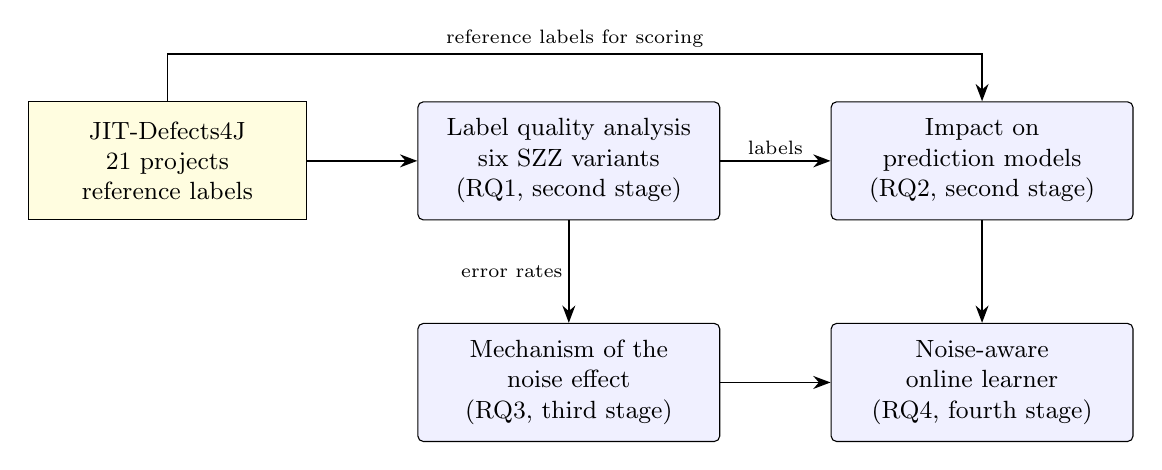
\begin{tikzpicture}[node distance=7mm and 14mm, font=\small,
  box/.style={draw, rounded corners=2pt, align=center, text width=36mm,
              minimum height=15mm, fill=blue!6},
  data/.style={draw, align=center, text width=33mm, minimum height=15mm, fill=yellow!12},
  arr/.style={-{Stealth[length=2.2mm]}, semithick},
  lab/.style={font=\scriptsize, fill=white, inner sep=1pt}]
\begin{scope}[every node/.append style={execute at begin node=\setstretch{1}}]
\node[data] (ref) {JIT-Defects4J\\21 projects\\reference labels};
\node[box, right=of ref] (s1) {Label quality analysis\\six SZZ variants\\(RQ1, second stage)};
\node[box, right=of s1] (s2) {Impact on\\prediction models\\(RQ2, second stage)};
\node[box, below=13mm of s1] (s3) {Mechanism of the\\noise effect\\(RQ3, third stage)};
\node[box, below=13mm of s2] (s4) {Noise-aware\\online learner\\(RQ4, fourth stage)};
\end{scope}
\draw[arr] (ref) -- (s1);
\draw[arr] (s1) -- node[lab, above=1pt] {labels} (s2);
\draw[arr] (s1) -- node[lab, left=1pt] {error rates} (s3);
\draw[arr] (s2) -- (s4);
\draw[arr] (s3) -- (s4);
\draw[arr] (ref.north) -- ++(0,6mm) -| node[lab, pos=0.25, above=1pt]
      {reference labels for scoring} (s2.north);
\end{tikzpicture}
\caption{Planned studies of the thesis and the research questions they
address.}
\label{fig:plan}
\end{figure}

The second stage consists of two studies that build on each other.

In the first study, the \emph{label quality analysis}, six SZZ variants will
be executed on the repositories of the 21 projects. Their labels will be
compared with the reference labels of the dataset. The result will be a
description of the errors of each variant, in particular its false positive
and false negative rates, and a set of SZZ labels for every commit. This
study addresses RQ1.

In the second study, the \emph{impact analysis}, prediction models will be
trained on the reference labels and on each of the six SZZ label sets. The
models will be evaluated in four evaluation settings, and their predictions
will be scored against the reference labels. This will show how much
performance is lost when a model is trained on SZZ labels, and how much the
evaluation setting itself changes the measured performance. This study
addresses RQ2.

The third stage will use the error rates measured in the second stage to set
up experiments in which the noise is controlled, and the fourth stage will use
the outcome of the third stage to design a learner that is less affected by
the noise.

The reference labels of the dataset are needed in every stage. In the first
study they are the standard against which the SZZ labels are assessed. In the
second study they are the standard against which the predictions are scored,
and they also provide the best available training labels, which serve as a
baseline for the models trained on SZZ labels.

\section{Generation of SZZ Labels}\label{sec:szz-generation}

The six SZZ variants of Table~\ref{tab:variants} will be executed with PySZZ
(version 2), the implementation released by Rosa et
al.~\cite{rosa2023szzvariants}. An existing implementation is preferred over
writing a new one, because it has been used in earlier studies and its
behaviour is documented. The configuration supplied with the tool will be
used for each variant. The filter that removes candidate commits made after
the bug report date will be switched off, because the dataset does not
contain the dates of the bug reports.

The input of the tool is a list of bug-fixing commits. The 5,453 commits of
the dataset whose FIX metric is set will be used for this purpose. The same
list will be given to all six variants, so that the differences between the
label sets come only from the variants and not from the selection of the
bug-fixing commits.

For every bug-fixing commit the tool returns the list of commits that the
variant considers defect-introducing. These mappings will be stored, since
they are also needed for the arrival times of the labels
(Section~\ref{sec:additions}). A commit will be labelled as defect-introducing
by a variant if it appears in the list of at least one bug-fixing commit, and
as clean otherwise. The labels will be joined with the dataset on the commit
identifier, so that all 27,319 commits receive a label from each variant.
Using the same set of commits for every variant is important, because
precision and recall are not comparable between variants when they are
computed on different subsets.

\section{Analysis of Label Quality}\label{sec:quality-method}

\subsection{Comparison with the reference labels}

For each variant, the SZZ label of every commit will be compared with its
reference label. The four possible outcomes are shown in
Table~\ref{tab:confusion}. A commit that is flagged by the variant and is
defect-introducing according to the reference is a true positive (TP). A
commit that is flagged by the variant but is clean according to the reference
is a false positive (FP). A commit that is not flagged but is
defect-introducing according to the reference is a false negative (FN), and a
commit that is clean according to both is a true negative (TN).

\begin{table}[htbp]
\centering\small
\caption{Outcomes of comparing an SZZ label with the reference label.}
\label{tab:confusion}
\begin{tabular}{@{}lcc@{}}
\toprule
 & \multicolumn{2}{c}{Reference label} \\
\cmidrule(l){2-3}
SZZ label & Defect-introducing & Clean \\
\midrule
Defect-introducing & TP & FP \\
Clean & FN & TN \\
\bottomrule
\end{tabular}
\end{table}

From these counts the following measures will be computed:
\begin{align}
\text{Precision} &= \frac{TP}{TP+FP}, &
\text{Recall} &= \frac{TP}{TP+FN}, &
F_1 &= \frac{2\cdot\text{Precision}\cdot\text{Recall}}{\text{Precision}+\text{Recall}}.
\end{align}
Precision is the fraction of the commits flagged by the variant that are
defect-introducing according to the reference. Recall is the fraction of the
reference defect-introducing commits that the variant finds. In addition, MCC
and Cohen's $\kappa$ between the SZZ labels and the reference labels will be
reported. Both are defined below.

\subsection{Noise rates}

For the study of label noise it is useful to describe a variant by the
probability with which it changes a reference label. Two rates are defined:
\begin{equation}
\rhoz = \frac{FP}{FP+TN}, \qquad \rhoo = \frac{FN}{FN+TP}.
\label{eq:rho}
\end{equation}
The rate $\rhoz$ is the fraction of the clean commits that the variant labels
as defect-introducing. It is called the false-alarm rate in this report. The
rate $\rhoo$ is the fraction of the defect-introducing commits that the
variant labels as clean. It is called the miss rate and equals one minus the
recall. A noise process that is described by these two rates is known as
class-conditional noise~\cite{natarajan2013noisy}. If both rates were equal,
the noise would be symmetric. Describing each variant by the pair
$(\rhoz,\rhoo)$ will show whether its noise is symmetric and, if not, which
type of error dominates.

Since the two classes have very different sizes, a rate and the corresponding
number of wrong labels must be distinguished. The clean class is about eleven
times larger than the defect-introducing class, so a small value of $\rhoz$
can correspond to a larger number of wrong labels than a large value of
$\rhoo$. Both the rates and the counts will therefore be reported.

\subsection{Agreement between variants}

The agreement between two label sets will be measured with Cohen's
$\kappa$~\cite{cohen1960kappa},
\begin{equation}
\kappa = \frac{p_o - p_e}{1 - p_e},
\end{equation}
where $p_o$ is the observed fraction of commits on which the two label sets
agree and $p_e$ is the fraction of agreement expected by chance, computed
from the proportions of positive labels in the two sets. The value will be
computed for every pair of variants and for every variant with the reference
labels. If the variants make their errors independently of each other, their
mutual agreement will not be much higher than their agreement with the
reference. A much higher mutual agreement would indicate that the variants
make the same errors.

\subsection{Variation across projects and sources of false negatives}

All measures will be computed for the whole dataset and also for each project
separately, to see how much the quality of the labels varies between
projects.

To understand why a variant misses defect-introducing commits, the false
negatives of each refined variant will be divided into two groups by
comparing them with B-SZZ. B-SZZ applies no filtering, so it traces every
line changed by the bug-fixing commits. A false negative of a refined variant
that is also a false negative of B-SZZ was missed already before any
filtering. A false negative that B-SZZ labels correctly was found by the
basic procedure and was then removed by the additional rules of the variant.
The sizes of the two groups will show how much of the miss rate of a variant
is caused by its own filtering.

\section{Prediction Models}\label{sec:models}

Three prediction models will be used in the impact analysis. They were chosen
to cover different levels of model complexity and both batch and online
learning. All three will use the same fourteen change metrics, so that
differences between them are not caused by different inputs.

\subsection{LApredict}

LApredict~\cite{zeng2021lapredict} is a logistic regression model that uses a
single feature, the number of added lines (LA). The feature will be
transformed as $\log(1+\mathrm{LA})$ and standardised, and the logistic
regression will be trained with class weights that are inversely proportional
to the class frequencies, so that both classes contribute equally to the
loss. A commit is predicted as defect-introducing when the predicted
probability is at least 0.5. The model represents a very simple learner with
only two parameters.

\subsection{Random forest model based on JITLine}

The second model follows the design of
JITLine~\cite{pornprasit2021jitline}: a random forest classifier combined
with oversampling of the minority class. A random
forest~\cite{breiman2001rf} with 100 trees will be trained on the fourteen
change metrics, which will be transformed as $\mathrm{sign}(x)\log(1+|x|)$ to
reduce their skewness. Before training, the minority class of the training
data will be oversampled with SMOTE~\cite{chawla2002smote} until both classes
have the same size. SMOTE creates new minority examples by interpolating
between an existing minority example and one of its nearest minority
neighbours.

A random forest produces a probability for each commit, and a decision
threshold is needed to turn it into a class. The threshold will be chosen on
the training data so that it maximises the G-mean
(Section~\ref{sec:measures}). To obtain probabilities that are not biased by
the model having seen the same commits, the training data will be divided
into consecutive blocks in time order, and each block will be predicted by a
model trained only on the blocks before it.

The original JITLine additionally uses features derived from the tokens of
the changed code. These will not be used here, so that all three models work
with the same features. For brevity this model is referred to as JITLine in
the rest of the report. It represents a learner with high capacity, which can
fit complex patterns in the training data.

\subsection{ORB}

The third model is ORB~\cite{cabral2019orb}, an online learner that was
designed for JIT-SDP with verification latency. It is an ensemble that is
updated with one training example at a time. The implementation planned for
this work has 20 base learners, each of which is a logistic regression model
trained by stochastic gradient descent. The features will be transformed in
the same way as for the random forest and standardised with running estimates
of their mean and variance.

When a training example $(x, y)$ arrives, each base learner is updated $k$
times with it, where $k$ is drawn from a Poisson distribution with parameter
$\lambda$. The value of $\lambda$ is what distinguishes the methods of this
family. In Online Bagging $\lambda = 1$. In OOB~\cite{wang2015oob}, $\lambda$
depends on the class of the example and on the current proportion $r_1$ of
positive examples, which is tracked as a decayed average,
\begin{equation}
r_1 \leftarrow \delta\, r_1 + (1-\delta)\,I(y=1), \qquad \delta = 0.99,
\end{equation}
where $I(y=1)$ is 1 if the example is positive and 0 otherwise. The rate is
then
\begin{equation}
\lambda_{\mathrm{OOB}} =
\begin{cases}
(1-r_1)/r_1 & \text{if } y=1 \text{ and } r_1 < 0.5,\\
r_1/(1-r_1) & \text{if } y=0 \text{ and } r_1 > 0.5,\\
1 & \text{otherwise.}
\end{cases}
\label{eq:oob}
\end{equation}
For example, if 10\% of the recent training examples are positive, a positive
example is presented on average nine times to each base learner.

ORB multiplies this rate by a boosting factor $b$ that depends on the recent
predictions of the model. Let $\bar{p}$ be a moving average of the
predictions (1 for defect-introducing, 0 for clean), which is updated after
every prediction as $\bar{p} \leftarrow \theta\,\bar{p} + (1-\theta)\,\hat{y}$
with $\theta = 0.4$. If the model predicts the positive class less often than
the proportion of positive examples it has seen ($\bar{p} < r_1$), positive
training examples are boosted. If it predicts the positive class more often
($\bar{p} > r_1$), negative training examples are boosted:
\begin{equation}
b =
\begin{cases}
l_0\,\dfrac{m^{\bar{p}} - m^{r_1}}{1 - m^{r_1}} + 1 & \text{if } y=1 \text{ and } \bar{p} < r_1,\\[2.2ex]
l_1\,\dfrac{n^{1-\bar{p}} - n^{1-r_1}}{1 - n^{1-r_1}} + 1 & \text{if } y=0 \text{ and } \bar{p} > r_1,\\[1.6ex]
1 & \text{otherwise,}
\end{cases}
\label{eq:orb}
\end{equation}
with the parameter values $l_0 = 10$, $l_1 = 12$, $m = 1.5$ and $n = 3$
proposed by the authors of ORB~\cite{cabral2019orb}. The final rate is
$\lambda = \lambda_{\mathrm{OOB}} \cdot b$. A commit is predicted as
defect-introducing when the majority of the base learners predict it so.

It can be seen from Equations~\ref{eq:oob} and~\ref{eq:orb} that the amount
of oversampling depends on the number of positive labels received and on the
predictions of the model, but not on whether the labels are correct. ORB
represents the online learners that are used when the commit stream is
processed in a realistic way.

\section{Evaluation Settings}\label{sec:settings}

The models will be evaluated in four settings, which are illustrated in
Figure~\ref{fig:settings}. They are ordered from the least to the most
realistic.

\begin{figure}[htbp]
\centering
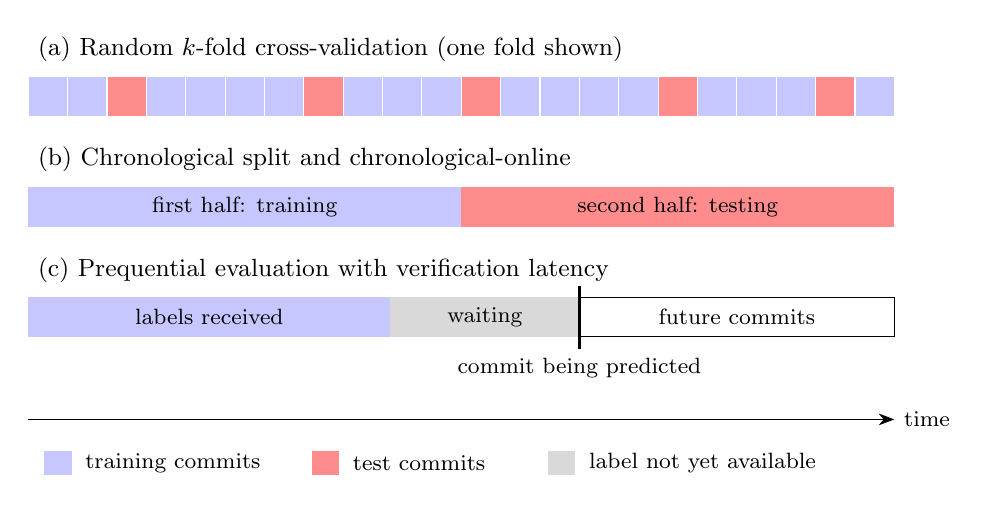
\begin{tikzpicture}[font=\footnotesize, x=1cm, y=1cm]
\def\w{11}
% (a) random k-fold
\node[anchor=west, font=\small] at (0,5.55) {(a) Random $k$-fold cross-validation (one fold shown)};
\foreach \i in {0,...,21} {
  \pgfmathtruncatemacro{\istest}{(\i==2 || \i==7 || \i==11 || \i==16 || \i==20) ? 1 : 0}
  \ifnum\istest=1
    \fill[red!45] (\i*0.5,4.7) rectangle ++(0.5,0.5);
  \else
    \fill[blue!22] (\i*0.5,4.7) rectangle ++(0.5,0.5);
  \fi
  \draw[white] (\i*0.5,4.7) rectangle ++(0.5,0.5);
}
% (b) chronological
\node[anchor=west, font=\small] at (0,4.15) {(b) Chronological split and chronological-online};
\fill[blue!22] (0,3.3) rectangle (5.5,3.8);
\fill[red!45] (5.5,3.3) rectangle (\w,3.8);
\node at (2.75,3.55) {first half: training};
\node at (8.25,3.55) {second half: testing};
% (c) prequential
\node[anchor=west, font=\small] at (0,2.75) {(c) Prequential evaluation with verification latency};
\fill[blue!22] (0,1.9) rectangle (4.6,2.4);
\fill[gray!30] (4.6,1.9) rectangle (7.0,2.4);
\draw (7.0,1.9) rectangle (\w,2.4);
\draw[thick] (7.0,1.75) -- (7.0,2.55);
\node at (2.3,2.15) {labels received};
\node at (5.8,2.15) {waiting};
\node at (9.0,2.15) {future commits};
\node[anchor=north] at (7.0,1.75) {commit being predicted};
% time axis and legend
\draw[-{Stealth[length=2mm]}] (0,0.85) -- (\w,0.85) node[right] {time};
\fill[blue!22] (0.2,0.15) rectangle ++(0.35,0.3); \node[anchor=west] at (0.6,0.3) {training commits};
\fill[red!45] (3.6,0.15) rectangle ++(0.35,0.3); \node[anchor=west] at (4.0,0.3) {test commits};
\fill[gray!30] (6.6,0.15) rectangle ++(0.35,0.3); \node[anchor=west] at (7.0,0.3) {label not yet available};
\end{tikzpicture}
\caption{The evaluation settings. The commits of a project are ordered by
time from left to right.}
\label{fig:settings}
\end{figure}

\paragraph{Random $k$-fold cross-validation.} The commits of a project are
divided at random into ten folds, stratified by the training label. Each fold
is used once for testing while the model is trained on the other nine. The
order of the commits is ignored, so the model is trained on commits that are
both older and newer than the test commits. This setting is included because
it is widely used in the literature. It will be applied to the two batch
models.

\paragraph{Chronological split.} The commits of a project are ordered by
time. The model is trained on the first half and tested on the second half.
The model never sees commits from the future, but it is assumed that the
labels of all training commits are known at the time of training. This
setting will also be applied to the two batch models.

\paragraph{Chronological-online.} This setting uses the same split for ORB.
The online learner processes the commits of the first half one by one with
their labels and is then kept fixed while it predicts the second half. It
makes it possible to compare ORB with the batch models on the same test
commits.

\paragraph{Prequential evaluation with verification latency.} The commits are
processed in time order. Each commit is first predicted by the current model.
Its label is given to the model for training only at the time at which it
would have become available in practice. The details are given in the next
section. The model is updated continuously over the whole stream. This
setting is the closest to the actual use of a JIT-SDP model and will be
applied to ORB.

\section{Simulation of Verification Latency}\label{sec:latency-method}

In the prequential setting the labels will be delivered to the learner
according to the procedure of Cabral et al.~\cite{cabral2019orb} with a
waiting period of $W = 90$ days. Let $t$ be the time of a commit. Four cases
are distinguished according to the training label of the commit and the time
of the bug-fixing commit linked to it (Section~\ref{sec:additions}). They are
shown in Figure~\ref{fig:latency-cases}.

\begin{enumerate}[leftmargin=*]
\item The commit is clean according to the training labels. Nothing is known
about it until the waiting period has passed. At time $t+W$ it is given to
the learner as a clean example.
\item The commit is defect-introducing and its fix is made before $t+W$. It
is given to the learner as a defect-introducing example at the time of the
fix.
\item The commit is defect-introducing and its fix is made after $t+W$. At
time $t+W$ no defect is known yet, so the commit is given to the learner as
a clean example. At the time of the fix it is given again, this time as a
defect-introducing example.
\item The commit is defect-introducing according to the training labels, but
no fix date is available for it. It is given to the learner as a clean
example at $t+W$ and is never corrected.
\end{enumerate}

\begin{figure}[htbp]
\centering
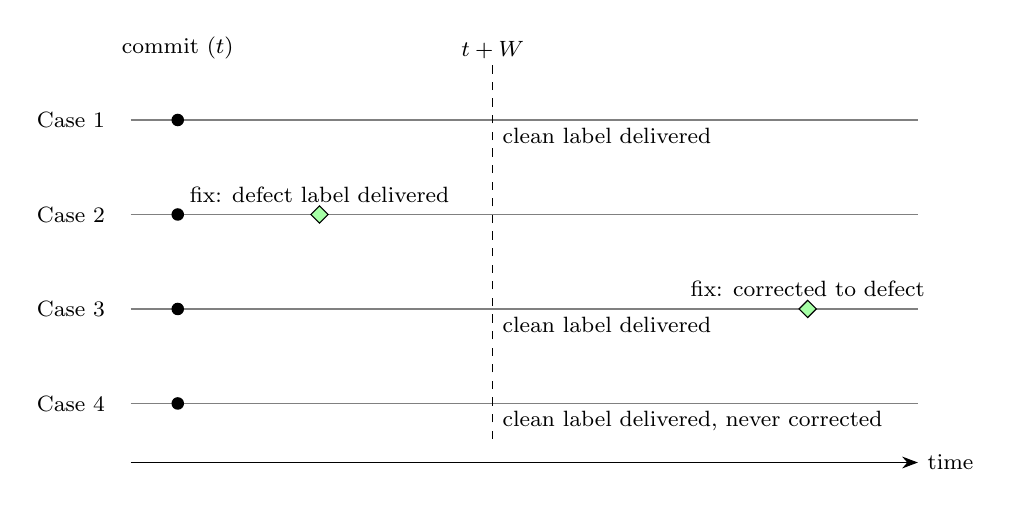
\begin{tikzpicture}[font=\footnotesize, x=1cm, y=1cm,
  ev/.style={circle, fill=black, inner sep=1.6pt},
  fix/.style={diamond, draw, fill=green!35, inner sep=1.6pt}]
\foreach \y/\lab in {3.6/Case 1, 2.4/Case 2, 1.2/Case 3, 0/Case 4} {
  \draw[gray] (1.6,\y) -- (11.6,\y);
  \node[anchor=east] at (1.4,\y) {\lab};
  \node[ev] at (2.2,\y) {};
}
\draw[dashed] (6.2,-0.45) -- (6.2,4.3);
\node[anchor=south] at (2.2,4.25) {commit ($t$)};
\node[anchor=south] at (6.2,4.25) {$t+W$};
% case 1
\node[anchor=north west, inner sep=2pt] at (6.25,3.58) {clean label delivered};
% case 2
\node[fix] at (4.0,2.4) {};
\node[anchor=south, inner sep=3pt] at (4.0,2.44) {fix: defect label delivered};
% case 3
\node[anchor=north west, inner sep=2pt] at (6.25,1.18) {clean label delivered};
\node[fix] at (10.2,1.2) {};
\node[anchor=south, inner sep=3pt] at (10.2,1.24) {fix: corrected to defect};
% case 4
\node[anchor=north west, inner sep=2pt] at (6.25,-0.02) {clean label delivered, never corrected};
\draw[-{Stealth[length=2mm]}] (1.6,-0.75) -- (11.6,-0.75) node[right] {time};
\end{tikzpicture}
\caption{Delivery of training labels under verification latency. In case 3
the learner first receives a wrong clean label, which is corrected when the
defect is fixed.}
\label{fig:latency-cases}
\end{figure}

Cases 3 and 4 are the ones in which the learner is trained on a wrong label
because of the delay. In case 3 the error is temporary. In case 4 it is
permanent. These errors occur with every label source, including the
reference labels, and they concern only defect-introducing commits. They add
to whatever errors the labels themselves contain.

The prediction for a commit is made at time $t$ and is scored at once, using
the label against which the model is evaluated (Section~\ref{sec:scoring}).
The scoring is not delayed, because its purpose is to measure the quality of
the predictions and not to simulate what a user of the model would know.
Algorithm~\ref{alg:prequential} summarises the procedure.

\begin{algorithm}[htbp]
\caption{Prequential evaluation with verification latency}
\label{alg:prequential}
\begin{algorithmic}[1]
\Require commits $c_1,\dots,c_N$ of a project in time order, with features
$x_i$, time $t_i$, training label $y_i$, evaluation label $e_i$ and fix time
$f_i$ (if available); waiting period $W$; online learner $M$
\State $Q \gets$ empty priority queue of pending training examples, ordered by delivery time
\For{$i = 1$ to $N$}
  \While{$Q$ is not empty and the earliest delivery time in $Q$ is at most $t_i$}
    \State remove the earliest example $(x_j, y)$ from $Q$ and update $M$ with it
  \EndWhile
  \State $\hat{y}_i \gets$ prediction of $M$ for $x_i$
  \State update the evaluation measures with $(e_i, \hat{y}_i)$
  \If{$y_i = 1$ and $f_i$ is available}
    \If{$f_i \le t_i + W$}
      \State add $(x_i, 1)$ to $Q$ with delivery time $f_i$
    \Else
      \State add $(x_i, 0)$ to $Q$ with delivery time $t_i + W$
      \State add $(x_i, 1)$ to $Q$ with delivery time $f_i$
    \EndIf
  \Else
    \State add $(x_i, 0)$ to $Q$ with delivery time $t_i + W$
  \EndIf
\EndFor
\end{algorithmic}
\end{algorithm}

\section{Scoring of the Predictions}\label{sec:scoring}

The predictions of a model can be compared with two different labels.

\paragraph{Scoring against the reference labels.} The predictions are
compared with the reference labels of the test commits. These labels are
never used for training when the model is trained on SZZ labels. The result
shows how well the model identifies the commits that are defect-introducing
according to the best available standard. This will be the main way of
scoring in this work.

\paragraph{Scoring against the training labels.} The predictions are
compared with the labels of the same SZZ variant that was used for training.
This is what is done in the literature, where only one set of labels is
available. It is called \emph{self-scoring} in this report.

For a model trained on SZZ labels both scores will be computed from the same
predictions. The difference between them will show how much the usual way of
scoring overestimates or underestimates the performance with respect to the
reference. For a model trained on the reference labels the two scores are the
same by definition.

\section{Performance Measures}\label{sec:measures}

The main performance measure will be the Matthews correlation
coefficient~\cite{matthews1975mcc},
\begin{equation}
\mathrm{MCC} = \frac{TP\cdot TN - FP\cdot FN}
{\sqrt{(TP+FP)(TP+FN)(TN+FP)(TN+FN)}},
\end{equation}
where the four counts are now obtained by comparing the predictions with the
evaluation labels. MCC ranges from $-1$ to $+1$. It is 0 for a model that
predicts at random or assigns all commits to one class, and it is high only
if the model performs well on both classes. It was chosen because of the
class imbalance: a model that predicts every commit as clean would reach an
accuracy of 91.5\% on this dataset but has an MCC of 0. MCC has also been
recommended for defect prediction in place of the
F-measure~\cite{yao2020mcc,chicco2020mcc}.

As a second measure the G-mean will be reported, which is the geometric mean
of the recall on the two classes,
\begin{equation}
\text{G-mean} = \sqrt{\frac{TP}{TP+FN}\cdot\frac{TN}{TN+FP}}.
\end{equation}
It is commonly used in online JIT-SDP~\cite{cabral2019orb} and becomes zero
when one of the classes is not recognised at all.

In the prequential setting the performance is not a single value, since the
model changes during the stream. The usual practice is to compute the
measures from a confusion matrix with a fading
factor~\cite{gama2013prequential}. Before each update, the four counts are
multiplied by a factor $f < 1$, and then the count that corresponds to the new
prediction is increased by one. Older predictions thus have less weight. With
$f = 0.99$ the weights add up to $1/(1-f) = 100$, so the matrix effectively
describes the last hundred commits. The MCC computed from this matrix changes
along the stream. Two summaries of it will be reported: its value at the end
of the stream, and its mean over the whole stream. The convergence result of
Gama et al.\ for the faded error rate does not carry over to MCC, so neither
summary can be taken as the standard one, and the sensitivity of the
conclusions to the fading factor will be examined.

\section{Statistical Analysis}\label{sec:stats}

Each configuration will be run with ten random seeds on each of the 21
projects. The seeds affect the random forest, the oversampling, the
assignment of commits to folds and the Poisson draws of ORB. Runs with
different seeds on the same project are not independent observations, because
they use the same data. For every configuration the results of the ten seeds
will therefore be averaged for each project first, and the statistical tests
will be carried out on the 21 project-level values. All comparisons will be
paired by project.

Let $d_1,\dots,d_{21}$ be the differences between two conditions for the 21
projects. The following quantities will be reported for each comparison.

\paragraph{Wilcoxon signed-rank test.} The null hypothesis that the
differences are symmetric around zero will be tested with the Wilcoxon
signed-rank test~\cite{wilcoxon1945}. The absolute differences are ranked,
and the sum $W^{+}$ of the ranks of the positive differences and the sum
$W^{-}$ of the ranks of the negative differences are computed. The test is
non-parametric and does not assume that the differences are normally
distributed, which cannot be assumed for MCC values of 21 projects.

\paragraph{Rank-biserial correlation.} As a measure of how consistently the
projects point in the same direction, the matched-pairs rank-biserial
correlation will be used,
\begin{equation}
r = \frac{W^{+} - W^{-}}{W^{+} + W^{-}}.
\end{equation}
It is $+1$ if all differences are positive, $-1$ if all are negative, and 0
if the positive and negative ranks balance.

\paragraph{Hodges--Lehmann estimate.} The size of the difference will be
estimated with the Hodges--Lehmann estimator~\cite{hodges1963}, which is the
median of all pairwise averages $(d_i + d_j)/2$ with $i \le j$. It is the
estimate of location that belongs to the signed-rank test and is less
sensitive to single extreme projects than the mean. A 95\% confidence
interval for it will be obtained with the percentile
bootstrap~\cite{efron1979bootstrap}, by resampling the 21 projects with
replacement.

\paragraph{Correction for multiple comparisons.} The study involves many
comparisons, and some of them would be expected to be significant by chance.
The $p$-values will therefore be adjusted with the method of
Holm~\cite{holm1979}. For $m$ tests with ordered $p$-values
$p_{(1)} \le \dots \le p_{(m)}$, the adjusted value of the $i$-th one is
\begin{equation}
\tilde{p}_{(i)} = \max_{j \le i}\,\min\bigl(1,\,(m-j+1)\,p_{(j)}\bigr).
\end{equation}
The correction will be applied over all tests of the study together, and a
significance level of 0.05 will be used.

\section{Experimental Setup}

The experiment of the impact analysis combines the three models with the
seven label sources, the evaluation settings applicable to each model and
the two ways of scoring. Table~\ref{tab:design} summarises the factors. For
each project and seed there are 78 configurations: each of the two batch
models is evaluated in two settings with seven label sources scored against
the reference and six scored against the training labels, and the same holds
for ORB with its two settings. With 21 projects and ten seeds this gives
$78 \times 21 \times 10 = 16{,}380$ evaluation runs.

\begin{table}[htbp]
\centering\small
\caption{Factors of the experiment in the impact analysis.}
\label{tab:design}
\begin{tabularx}{\linewidth}{@{}l>{\raggedright\arraybackslash}X@{}}
\toprule
Factor & Levels \\
\midrule
Model & LApredict, JITLine (batch models); ORB (online model) \\
Training labels & Reference labels; labels of B-SZZ, AG-SZZ, MA-SZZ, L-SZZ,
R-SZZ and RA-SZZ \\
Evaluation setting & Random 10-fold cross-validation and chronological split
(batch models); chronological-online and prequential with verification
latency (ORB) \\
Scoring & Against the reference labels; against the training labels \\
Projects & 21 \\
Random seeds & 10 \\
\bottomrule
\end{tabularx}
\end{table}

The experiments will be implemented in Python with scikit-learn for the batch
models and imbalanced-learn for SMOTE. The online learner and the prequential
evaluation will be implemented for this work. Every table and figure will be
produced by a script from the stored outputs of the experiments, so that the
results can be regenerated.

\section{Approach for the Third and Fourth Stages}\label{sec:later}

The methodology of the later stages depends on the results of the second
stage, so only its outline is given here.

The third stage addresses RQ3. If the second stage shows that SZZ labels
reduce the performance of an online learner, the next question is which type
of labelling error causes the loss. Two label sources differ in the number of
false positives, in the number of false negatives and in the arrival times of
the labels at the same time, so a comparison of label sources cannot answer
this question. Experiments are therefore planned in which one property of the
labels is changed at a time. Label noise will be injected into the reference
labels at the rates measured in the second stage, and the labels of an SZZ
variant will be corrected with the help of the reference labels, one type of
error at a time. It will also be examined whether the oversampling used by
online learners for imbalanced streams (Section~\ref{sec:models}) increases
the effect of wrongly labelled positive examples.

The fourth stage addresses RQ4. Based on the findings of the third stage, a
modification of the online learner will be designed that makes it less
sensitive to the type of error found to be harmful. The modification has to
work without access to clean labels, since these are not available in
practice. It should improve the performance when the learner is trained on
SZZ labels, and it should not reduce the performance when the labels are
clean.

\section{Summary}

In the second stage, six SZZ variants will be run with PySZZ on the
bug-fixing commits of the dataset, and their labels will be compared with the
reference labels in terms of precision, recall, noise rates and agreement.
Three models of different complexity will then be trained on seven label
sources and evaluated in four settings, from random cross-validation to
prequential evaluation with verification latency. The predictions will be
scored against the reference labels and against the training labels, and the
comparisons will be tested at the level of projects with the Wilcoxon
signed-rank test and corrected for multiple comparisons. The third and fourth
stages will study the cause of the loss and a way to reduce it.

% ============================================================================
\chapter{Conclusion and Plan of Work}\label{ch:conclusion}
% ============================================================================

This chapter summarises the work done in the first stage and gives the plan
of work for the remaining stages of the thesis.

\section{Summary of the Work Done}

The thesis deals with the effect of the label noise introduced by the SZZ
algorithm on just-in-time software defect prediction. The work of the first
stage consisted of four parts.

First, the literature was reviewed. The review covered defect prediction at
the level of changes, the SZZ algorithm and its variants together with the
studies that evaluate them, the studies on label noise in defect data, the
evaluation of prediction models with respect to time and to the delayed
arrival of labels, online learning for imbalanced data streams, and learning
with noisy labels.

Second, the research gaps were identified and the objectives and research
questions were formulated. The review showed that the accuracy of SZZ, the
effect of label noise, time-aware evaluation and verification latency have
each been studied, but mostly separately. The noise of SZZ labels has not been
measured over complete project histories, models are tested against the same
labels on which they are trained, the effect of label noise has not been
separated from the effect of the evaluation procedure, and label noise has
not been studied under verification latency. Three objectives and four
research questions were derived from these gaps (Chapter~\ref{ch:gaps}).

Third, a dataset was selected and prepared. The JIT-Defects4J dataset was
chosen because it provides, for every commit of 21 projects, a label that was
derived from manually validated bug-fixing lines and not from the SZZ variants
under study. The construction of these labels was examined, and its
consequences for the planned comparisons were noted. The dataset was merged,
cleaned and ordered by time, and the repositories of the projects were
obtained.

Fourth, the methodology of the study was designed
(Chapter~\ref{ch:method}). It specifies how the SZZ labels will be generated
and assessed, which prediction models will be used, how they will be
evaluated with respect to time and to the delay of the labels, and how the
results will be tested.

\section{Plan of Work}\label{sec:plan}

The remaining work is planned in three stages. Table~\ref{tab:timeline}
gives the timeline.

In the second stage, the methodology of Chapter~\ref{ch:method} will be
carried out. The labels of the six SZZ variants will be generated and
compared with the reference labels, which addresses RQ1, and their effect on
prediction models will be measured in the four evaluation settings, which
addresses RQ2. With this stage the first two objectives will be met.

In the third stage, the cause of the loss will be studied with experiments in
which the label noise is controlled, which addresses RQ3. In the fourth stage
a noise-aware online learner will be designed and evaluated, which addresses
RQ4, and the writing of the thesis will be completed. These two stages meet
the third objective. Their outline is given in Section~\ref{sec:later}.

\begin{table}[htbp]
\centering\small
\caption{Timeline of the thesis work.}
\label{tab:timeline}
\begin{tabularx}{\linewidth}{@{}l>{\raggedright\arraybackslash}Xl@{}}
\toprule
Stage & Work & Status \\
\midrule
First & Literature survey; identification of research gaps; objectives and
research questions; selection and preparation of the dataset; design of the
methodology & Completed \\
Second & Generation of SZZ labels; label quality analysis (RQ1); impact on
prediction models under different evaluation settings (RQ2) & Planned \\
Third & Noise injection and label repair experiments; mechanism of the
noise effect (RQ3) & Planned \\
Fourth & Design and evaluation of a noise-aware online learner (RQ4); thesis
writing & Planned \\
\bottomrule
\end{tabularx}
\end{table}

% ------------------------------------------------------------- references
{\small\singlespacing
\begin{thebibliography}{99}
\addcontentsline{toc}{chapter}{References}
\setlength{\itemsep}{1pt}

\bibitem{hall2012slr}
T.~Hall, S.~Beecham, D.~Bowes, D.~Gray, and S.~Counsell, ``A systematic
literature review on fault prediction performance in software engineering,''
\emph{IEEE Transactions on Software Engineering}, vol.~38, no.~6,
pp.~1276--1304, 2012.

\bibitem{rathore2019study}
S.~S. Rathore and S.~Kumar, ``A study on software fault prediction
techniques,'' \emph{Artificial Intelligence Review}, vol.~51, no.~2,
pp.~255--327, 2019.

\bibitem{kamei2013jit}
Y.~Kamei, E.~Shihab, B.~Adams, A.~E. Hassan, A.~Mockus, A.~Sinha, and
N.~Ubayashi, ``A large-scale empirical study of just-in-time quality
assurance,'' \emph{IEEE Transactions on Software Engineering}, vol.~39, no.~6,
pp.~757--773, 2013.

\bibitem{mockus2000risk}
A.~Mockus and D.~M. Weiss, ``Predicting risk of software changes,'' \emph{Bell
Labs Technical Journal}, vol.~5, no.~2, pp.~169--180, 2000.

\bibitem{kim2008classifying}
S.~Kim, E.~J. Whitehead, Jr., and Y.~Zhang, ``Classifying software changes:
Clean or buggy?'' \emph{IEEE Transactions on Software Engineering}, vol.~34,
no.~2, pp.~181--196, 2008.

\bibitem{sliwerski2005szz}
J.~\'{S}liwerski, T.~Zimmermann, and A.~Zeller, ``When do changes induce
fixes?'' in \emph{Proceedings of the International Workshop on Mining Software
Repositories (MSR)}, 2005, pp.~1--5.

\bibitem{herbold2022tangling}
S.~Herbold, A.~Trautsch, B.~Ledel, \emph{et al.}, ``A fine-grained data set and
analysis of tangling in bug fixing commits,'' \emph{Empirical Software
Engineering}, vol.~27, no.~6, article 125, 2022.

\bibitem{dacosta2017maszz}
D.~A. da~Costa, S.~McIntosh, W.~Shang, U.~Kulesza, R.~Coelho, and A.~E.
Hassan, ``A framework for evaluating the results of the SZZ approach for
identifying bug-introducing changes,'' \emph{IEEE Transactions on Software
Engineering}, vol.~43, no.~7, pp.~641--657, 2017.

\bibitem{rosa2021oracle}
G.~Rosa, L.~Pascarella, S.~Scalabrino, R.~Tufano, G.~Bavota, M.~Lanza, and
R.~Oliveto, ``Evaluating SZZ implementations through a developer-informed
oracle,'' in \emph{Proceedings of the 43rd IEEE/ACM International Conference on
Software Engineering (ICSE)}, 2021.

\bibitem{falessi2020order}
D.~Falessi, J.~Huang, L.~Narayana, J.~F. Thai, and B.~Turhan, ``On the need of
preserving order of data when validating within-project defect classifiers,''
\emph{Empirical Software Engineering}, vol.~25, pp.~4805--4830, 2020.

\bibitem{tan2015online}
M.~Tan, L.~Tan, S.~Dara, and C.~Mayeux, ``Online defect prediction for
imbalanced data,'' in \emph{Proceedings of the 37th International Conference on
Software Engineering (ICSE)}, vol.~2, 2015, pp.~99--108.

\bibitem{cabral2019orb}
G.~G. Cabral, L.~L. Minku, E.~Shihab, and S.~Mujahid, ``Class imbalance
evolution and verification latency in just-in-time software defect
prediction,'' in \emph{Proceedings of the 41st International Conference on
Software Engineering (ICSE)}, 2019, pp.~666--676.

\bibitem{cabral2023reliable}
G.~G. Cabral and L.~L. Minku, ``Towards reliable online just-in-time software
defect prediction,'' \emph{IEEE Transactions on Software Engineering}, vol.~49,
no.~3, pp.~1342--1358, 2023.

\bibitem{zhao2023survey}
Y.~Zhao, K.~Damevski, and H.~Chen, ``A systematic survey of just-in-time
software defect prediction,'' \emph{ACM Computing Surveys}, vol.~55, no.~10,
pp.~1--35, 2023.

\bibitem{mcintosh2018moving}
S.~McIntosh and Y.~Kamei, ``Are fix-inducing changes a moving target? A
longitudinal case study of just-in-time defect prediction,'' \emph{IEEE
Transactions on Software Engineering}, vol.~44, no.~5, pp.~412--428, 2018.

\bibitem{hoang2019deepjit}
T.~Hoang, H.~K. Dam, Y.~Kamei, D.~Lo, and N.~Ubayashi, ``DeepJIT: An end-to-end
deep learning framework for just-in-time defect prediction,'' in
\emph{Proceedings of the 16th International Conference on Mining Software
Repositories (MSR)}, 2019.

\bibitem{hoang2020cc2vec}
T.~Hoang, H.~J. Kang, D.~Lo, and J.~Lawall, ``CC2Vec: Distributed
representations of code changes,'' in \emph{Proceedings of the 42nd
International Conference on Software Engineering (ICSE)}, 2020.

\bibitem{zeng2021lapredict}
Z.~Zeng, Y.~Zhang, H.~Zhang, and L.~Zhang, ``Deep just-in-time defect
prediction: How far are we?'' in \emph{Proceedings of the 30th ACM SIGSOFT
International Symposium on Software Testing and Analysis (ISSTA)}, 2021.

\bibitem{pornprasit2021jitline}
C.~Pornprasit and C.~Tantithamthavorn, ``JITLine: A simpler, better, faster,
finer-grained just-in-time defect prediction,'' in \emph{Proceedings of the
18th International Conference on Mining Software Repositories (MSR)}, 2021,
pp.~369--379.

\bibitem{yang2016effort}
Y.~Yang, Y.~Zhou, J.~Liu, Y.~Zhao, H.~Lu, L.~Xu, B.~Xu, and H.~Leung,
``Effort-aware just-in-time defect prediction: Simple unsupervised models
could be better than supervised models,'' in \emph{Proceedings of the 24th ACM
SIGSOFT International Symposium on Foundations of Software Engineering (FSE)},
2016, pp.~157--168.

\bibitem{rodriguez2020bugs}
G.~Rodr\'{\i}guez-P\'{e}rez, G.~Robles, A.~Serebrenik, A.~Zaidman, D.~M.
Germ\'{a}n, and J.~M. Gonz\'{a}lez-Barahona, ``How bugs are born: A model to
identify how bugs are introduced in software components,'' \emph{Empirical
Software Engineering}, vol.~25, pp.~1294--1340, 2020.

\bibitem{kim2006agszz}
S.~Kim, T.~Zimmermann, K.~Pan, and E.~J. Whitehead, Jr., ``Automatic
identification of bug-introducing changes,'' in \emph{Proceedings of the 21st
IEEE/ACM International Conference on Automated Software Engineering (ASE)},
2006, pp.~81--90.

\bibitem{davies2014rlszz}
S.~Davies, M.~Roper, and M.~Wood, ``Comparing text-based and dependence-based
approaches for determining the origins of bugs,'' \emph{Journal of Software:
Evolution and Process}, vol.~26, no.~1, pp.~107--139, 2014.

\bibitem{neto2018raszz}
E.~C. Neto, D.~A. da~Costa, and U.~Kulesza, ``The impact of refactoring changes
on the SZZ algorithm: An empirical study,'' in \emph{Proceedings of the 25th
IEEE International Conference on Software Analysis, Evolution and
Reengineering (SANER)}, 2018, pp.~380--390.

\bibitem{rodriguez2018szz}
G.~Rodr\'{\i}guez-P\'{e}rez, G.~Robles, and J.~M. Gonz\'{a}lez-Barahona,
``Reproducibility and credibility in empirical software engineering: A case
study based on a systematic literature review of the use of the SZZ
algorithm,'' \emph{Information and Software Technology}, vol.~99,
pp.~164--176, 2018.

\bibitem{rosa2023szzvariants}
G.~Rosa, L.~Pascarella, S.~Scalabrino, R.~Tufano, G.~Bavota, M.~Lanza, and
R.~Oliveto, ``A comprehensive evaluation of SZZ variants through a
developer-informed oracle,'' \emph{Journal of Systems and Software}, vol.~202,
article 111729, 2023.

\bibitem{herzig2013tangled}
K.~Herzig and A.~Zeller, ``The impact of tangled code changes,'' in
\emph{Proceedings of the 10th Working Conference on Mining Software
Repositories (MSR)}, 2013, pp.~121--130.

\bibitem{kim2011noise}
S.~Kim, H.~Zhang, R.~Wu, and L.~Gong, ``Dealing with noise in defect
prediction,'' in \emph{Proceedings of the 33rd International Conference on
Software Engineering (ICSE)}, 2011, pp.~481--490.

\bibitem{tantithamthavorn2015mislabelling}
C.~Tantithamthavorn, S.~McIntosh, A.~E. Hassan, A.~Ihara, and K.~Matsumoto,
``The impact of mislabelling on the performance and interpretation of defect
prediction models,'' in \emph{Proceedings of the 37th International Conference
on Software Engineering (ICSE)}, 2015, pp.~812--823.

\bibitem{fan2021mislabeled}
Y.~Fan, X.~Xia, D.~A. da~Costa, D.~Lo, A.~E. Hassan, and S.~Li, ``The impact of
changes mislabeled by SZZ on just-in-time defect prediction,'' \emph{IEEE
Transactions on Software Engineering}, vol.~47, no.~8, pp.~1559--1586, 2021.

\bibitem{gama2013prequential}
J.~Gama, R.~Sebasti\~{a}o, and P.~P. Rodrigues, ``On evaluating stream learning
algorithms,'' \emph{Machine Learning}, vol.~90, no.~3, pp.~317--346, 2013.

\bibitem{tabassum2020cross}
S.~Tabassum, L.~L. Minku, D.~Feng, G.~G. Cabral, and L.~Song, ``An
investigation of cross-project learning in online just-in-time software defect
prediction,'' in \emph{Proceedings of the 42nd International Conference on
Software Engineering (ICSE)}, 2020, pp.~554--565.

\bibitem{yao2020mcc}
J.~Yao and M.~Shepperd, ``Assessing software defection prediction performance:
Why using the Matthews correlation coefficient matters,'' in \emph{Proceedings
of the 24th International Conference on Evaluation and Assessment in Software
Engineering (EASE)}, 2020, pp.~120--129.

\bibitem{matthews1975mcc}
B.~W. Matthews, ``Comparison of the predicted and observed secondary structure
of T4 phage lysozyme,'' \emph{Biochimica et Biophysica Acta (BBA) -- Protein
Structure}, vol.~405, no.~2, pp.~442--451, 1975.

\bibitem{chicco2020mcc}
D.~Chicco and G.~Jurman, ``The advantages of the Matthews correlation
coefficient (MCC) over F1 score and accuracy in binary classification
evaluation,'' \emph{BMC Genomics}, vol.~21, article 6, 2020.

\bibitem{cohen1960kappa}
J.~Cohen, ``A coefficient of agreement for nominal scales,'' \emph{Educational
and Psychological Measurement}, vol.~20, no.~1, pp.~37--46, 1960.

\bibitem{landis1977kappa}
J.~R. Landis and G.~G. Koch, ``The measurement of observer agreement for
categorical data,'' \emph{Biometrics}, vol.~33, no.~1, pp.~159--174, 1977.

\bibitem{oza2001onlinebagging}
N.~C. Oza and S.~Russell, ``Online bagging and boosting,'' in
\emph{Proceedings of the 8th International Workshop on Artificial Intelligence
and Statistics (AISTATS)}, 2001, pp.~229--236.

\bibitem{wang2015oob}
S.~Wang, L.~L. Minku, and X.~Yao, ``Resampling-based ensemble methods for
online class imbalance learning,'' \emph{IEEE Transactions on Knowledge and
Data Engineering}, vol.~27, no.~5, pp.~1356--1368, 2015.

\bibitem{natarajan2013noisy}
N.~Natarajan, I.~S. Dhillon, P.~Ravikumar, and A.~Tewari, ``Learning with noisy
labels,'' in \emph{Advances in Neural Information Processing Systems (NIPS)},
2013.

\bibitem{han2018coteaching}
B.~Han, Q.~Yao, X.~Yu, G.~Niu, M.~Xu, W.~Hu, I.~Tsang, and M.~Sugiyama,
``Co-teaching: Robust training of deep neural networks with extremely noisy
labels,'' in \emph{Advances in Neural Information Processing Systems
(NeurIPS)}, 2018.

\bibitem{northcutt2021confident}
C.~G. Northcutt, L.~Jiang, and I.~L. Chuang, ``Confident learning: Estimating
uncertainty in dataset labels,'' \emph{Journal of Artificial Intelligence
Research}, vol.~70, pp.~1373--1411, 2021.

\bibitem{keshavarz2022apachejit}
H.~Keshavarz and M.~Nagappan, ``ApacheJIT: A large dataset for just-in-time
defect prediction,'' in \emph{Proceedings of the 19th International Conference
on Mining Software Repositories (MSR)}, 2022.

\bibitem{mahbub2023defectors}
P.~Mahbub, O.~Shuvo, and M.~M. Rahman, ``Defectors: A large, diverse Python
dataset for defect prediction,'' in \emph{Proceedings of the 20th International
Conference on Mining Software Repositories (MSR)}, 2023.

\bibitem{ni2022jitdefects4j}
C.~Ni, W.~Wang, K.~Yang, X.~Xia, K.~Liu, and D.~Lo, ``The best of both worlds:
Integrating semantic features with expert features for defect prediction and
localization,'' in \emph{Proceedings of the 30th ACM Joint European Software
Engineering Conference and Symposium on the Foundations of Software
Engineering (ESEC/FSE)}, 2022, pp.~672--683.

\bibitem{breiman2001rf}
L.~Breiman, ``Random forests,'' \emph{Machine Learning}, vol.~45, no.~1,
pp.~5--32, 2001.

\bibitem{chawla2002smote}
N.~V. Chawla, K.~W. Bowyer, L.~O. Hall, and W.~P. Kegelmeyer, ``SMOTE:
Synthetic minority over-sampling technique,'' \emph{Journal of Artificial
Intelligence Research}, vol.~16, pp.~321--357, 2002.

\bibitem{wilcoxon1945}
F.~Wilcoxon, ``Individual comparisons by ranking methods,'' \emph{Biometrics
Bulletin}, vol.~1, no.~6, pp.~80--83, 1945.

\bibitem{hodges1963}
J.~L. Hodges and E.~L. Lehmann, ``Estimates of location based on rank tests,''
\emph{The Annals of Mathematical Statistics}, vol.~34, no.~2, pp.~598--611,
1963.

\bibitem{efron1979bootstrap}
B.~Efron, ``Bootstrap methods: Another look at the jackknife,'' \emph{The
Annals of Statistics}, vol.~7, no.~1, pp.~1--26, 1979.

\bibitem{holm1979}
S.~Holm, ``A simple sequentially rejective multiple test procedure,''
\emph{Scandinavian Journal of Statistics}, vol.~6, no.~2, pp.~65--70, 1979.

\end{thebibliography}
}

\end{document}
